\documentclass[preprint,12pt,authoryear]{elsarticle}

\usepackage{lmodern}
\usepackage{amsmath,amssymb}
\usepackage{graphicx}
\usepackage{booktabs}
\usepackage{multirow}
\usepackage{float}
\usepackage[section]{placeins}
\usepackage{xcolor}
\usepackage[hidelinks,hypertexnames=false]{hyperref}
\usepackage{algorithm}
\usepackage{algorithmic}
\usepackage{pgfplots}
\pgfplotsset{compat=1.18}
\setlength{\emergencystretch}{2em}
% Parenthetical citations by default; explicit \citet remains narrative.
\let\cite\citep

\journal{Journal of Network and Computer Applications}

\graphicspath{{./}}

\newcommand{\ours}{CARE}  % Collapse-Aware REpair
\newcommand{\ie}{\textit{i.e.}}
\newcommand{\eg}{\textit{e.g.}}
\newcommand{\etal}{\textit{et al.}\@}

\begin{document}

\begin{frontmatter}

\title{Collapse-Aware Repair for Encrypted Traffic Classification under Concept Drift}

\author[a]{Junwei Xiao}
\ead{xjw20528@stu2024.jnu.edu.cn}
\author[b]{Xiaobo Jin}
\ead{Xiaobo.Jin@xjtlu.edu.cn}
\author[c]{Xiucheng Wu}
\ead{mwu@coremail.cn}
\author[a]{Dongjie Liu\corref{cor1}}
\ead{djliu@jnu.edu.cn}
\cortext[cor1]{Corresponding author. ORCID: \url{https://orcid.org/0009-0001-8405-166X}.}
\address[a]{College of Cyber Security, Jinan University, No. 855 Xingye Avenue East, Panyu District, Guangzhou, Guangdong 511443, China}
\address[b]{Department of Intelligent Science, School of Advanced Technology, Xi'an Jiaotong-Liverpool University, 111 Ren'ai Road, Suzhou Dushu Lake Science and Education Innovation District, Suzhou Industrial Park, Suzhou, Jiangsu 215123, P.R. China}
\address[c]{Coremail, Floors 7--10, Building 3, Chuangzhi Tower, No. 28 Qinglan Street, Guangzhou Higher Education Mega Center, Guangzhou, Guangdong 510006, China}

\begin{abstract}
Encrypted-traffic classifiers degrade as traffic distributions evolve, yet aggregate metrics can conceal severe class-specific failures. We formalize absorber collapse, a class-asymmetric failure in which dominant classes absorb predictions from victim classes and drive their recall toward zero. On CESNET-TLS-Year22, 12 of 178 classes collapse within nine months, while five tested traffic-adapted test-time adaptation methods leave collapse-class F1 below 0.031. We propose Collapse-Aware Repair (CARE), a label-efficient maintenance framework that combines an unsupervised class-health monitor with head-only repair using actively selected target labels, all-class reference replay, and knowledge distillation. Monitoring supports diagnosis; it does not guide the default query selector. Using Batch Active Learning by Diverse Gradient Embeddings (BADGE), CARE raises macro-F1 from 0.629 to 0.700 and collapse-class F1 from 0.028 to 0.332 with 1{,}000 target labels under strict query-excluded evaluation over five repair seeds, while retaining stable-class F1 near the static level (0.894 versus 0.903). Improvements persist across the evaluated drift periods and architectures. A QUIC cross-protocol stress test identifies limits under more severe shift. CARE provides a class-aware approach to maintaining reliable predictions with scarce supervision; it does not guarantee recovery of every class, and cross-site deployment remains unvalidated.
\end{abstract}

\begin{keyword}
Encrypted traffic classification \sep Concept drift \sep Class collapse \sep Label-efficient maintenance \sep Active learning
\end{keyword}

\end{frontmatter}

% ============================================================
\section{Introduction}
\label{sec:intro}

% P1: Problem - drift in traffic classifiers
Deep learning has become the dominant approach for encrypted traffic classification, achieving impressive accuracy on benchmark datasets~\cite{lin2022etbert, zhao2023yatc, pacheco2019towards, wang2019survey}.
However, a growing body of evidence shows that these classifiers degrade rapidly after deployment.
Prior studies report frequent class drift on CESNET-TLS-Year22~\cite{soukup2025drift} and substantial F1 degradation over time on Internet service provider (ISP)-scale data~\cite{malekghaini2023drift}.
The causes are diverse: application updates alter protocol behavior, Transport Layer Security (TLS) certificate rotations change handshake fingerprints, and content delivery network (CDN) migrations shift Internet Protocol (IP) ranges and packet-size distributions~\cite{soukup2025drift, lu2019learning, gama2014survey}.

For an AI prediction system, acceptable aggregate performance does not ensure that every class remains usable. Encrypted-traffic classification illustrates this reliability problem: predictions can support quality-of-service monitoring, anomaly triage, capacity planning, and policy enforcement~\cite{rezaei2019deep,pacheco2019towards}, yet a collapsed class could be systematically omitted from the resulting decisions. This motivates class-aware maintenance that explicitly measures class recovery alongside preservation of the remaining classes under a limited labeling budget.

% P2: Existing solutions and their limitations
Existing approaches to this problem span three categories.
Label-free self-evolving adaptation uses high-confidence pseudo-labels to update a model without human annotation~\cite{chen2025selfevolving}, but its behavior on collapsed classes has not been established.
Unsupervised test-time adaptation (TTA) from computer vision~\cite{wang2021tent, niu2022eata, niu2023sar} avoids labeling but does not repair collapsed classes under our tested traffic adaptations.
Standard active learning~\cite{settles2009active, sener2018coreset, ash2020badge} can select informative samples, but generic strategies are not designed for the specific failure mode we identify.
This motivates \textit{class-aware, label-efficient maintenance}: diagnosing collapse and assessing whether a small supervised update recovers affected classes while preserving the rest.

% P3: Our finding - absorber-collapse pattern
We formalize and systematically characterize a previously underexamined class-asymmetric failure pattern that we term the \textit{absorber-collapse pattern}.
Our systematic confusion analysis on the CESNET-TLS-Year22 dataset~\cite{hynek2024cesnet} shows that performance degradation is not uniform across classes.
Instead, a small number of dominant ``absorber'' classes systematically attract predictions away from ``victim'' classes, causing the victims to collapse to near-zero recall within a short deployment period.
Traffic-adapted TTA variants, including SAR~\cite{niu2023sar} and NOTE~\cite{gong2022note}, do not materially recover these collapsed classes under our implementations.

% P4: Our solution - CARE
In response to these limitations, we propose \ours{} (Collapse-Aware REpair), a collapse-aware, operator-in-the-loop maintenance framework for encrypted-traffic classifiers.
Unlike unsupervised TTA, which adapts without collapse-specific supervision, and standard active learning, which selects informative samples without explicitly evaluating class-collapse recovery, \ours{} couples class-health diagnosis with a repair pipeline assessed for both collapse recovery and stable-class preservation.

\ours{} shifts maintenance from confidence-driven, label-free adaptation to targeted, label-efficient repair.
A multi-signature unsupervised monitor ranks class-level risk for operator review.
Once a repair cycle is approved, Margin or BADGE selects a small batch of informative target samples for labeling; \ours{} then updates only the classification head using the labeled target features, all-class reference-period replay, and knowledge distillation.
This design addresses two linked objectives: recovering collapsed classes and limiting forgetting across the remaining stable classes.

% P5: Engineering workflow
\ours{} is formulated as a scheduled offline maintenance procedure rather than an autonomous online adaptation rule.
In the proposed workflow, the deployed model continues serving while an operator reviews monitoring alerts, approves label acquisition and repair, and validates a candidate head before activation; the original model can be retained for rollback.
Freezing the encoder limits the scope of optimization and avoids full-model retraining.
The bounded head-only update and operator-reviewed activation process make the framework suitable for periodic offline maintenance, while production-field validation remains future work.

% P6: Evaluation and generalization
Our evaluation is designed to test both repair effectiveness and its operating limits.
The main experiments use strict query exclusion, repeated runs, collapse/stable F1, and per-class recovery status; additional matched-holdout experiments compare \ours{} with a Chen-inspired self-evolving baseline, while broader comparisons cover TTA variants, standard active-learning selectors, and adapted continual-learning or drift methods.
Further studies examine different drift periods, model backbones, and a QUIC cross-protocol stress test to assess transferability and delimit the framework's operating range.

Together, these results assess class recovery and preservation within one diagnosis-and-repair procedure.

The study makes three contributions to class-aware maintenance.

First, we formalize absorber collapse and provide longitudinal, per-class evidence together with two descriptive Fisher signatures.

Second, we develop and evaluate a label-efficient repair framework that integrates diagnostic monitoring, active target-label selection, all-class reference replay, and head-only updating in an operator-reviewed offline workflow. Its contribution is this maintenance formulation and integration, using established active-learning and distillation techniques.

Third, we evaluate class recovery and stable-class damage with strict query exclusion, matched holdouts, comparative baselines, runtime measurements, multiple drift periods and backbones, and a QUIC cross-protocol stress test, while reporting the resulting operating limits.


% ============================================================
\section{Related Work}
\label{sec:related}

Encrypted traffic classifiers are intrinsically non-stationary after deployment because the packet-sequence statistics on which they rely change with applications, protocols, and network infrastructure~\cite{rezaei2019deep,soukup2025drift,malekghaini2023drift}. Longitudinal studies have documented the resulting degradation: \citet{soukup2025drift} identified 28 frequently drifting classes on CESNET-TLS-Year22; \citet{malekghaini2023drift} observed that ``web is the class most of the misclassified flows are confused with''; and \citet{jerabek2025eval} showed that random splitting inflates performance by at least 3.5 percentage points relative to time-based evaluation. Yet prior work has largely pursued two broad remedies---label-free adaptation and label-assisted maintenance---without formulating the high-confidence, class-asymmetric absorber-collapse failure studied here. This omission matters because acceptable aggregate performance can coexist with near-zero recall for a small set of victim classes.

Label-free test-time adaptation (TTA) includes Tent~\cite{wang2021tent}, EATA~\cite{niu2022eata}, SAR~\cite{niu2023sar}, CoTTA~\cite{wang2022cotta}, and NOTE~\cite{gong2022note}. Tent minimizes prediction entropy, while the other methods add different sample-selection, optimization, or teacher-update mechanisms for broader target-domain adaptation. The key mismatch for absorber collapse lies in the adaptation signal: when an absorber confidently captures a victim's predictions, entropy is low, confidence is high, and a pseudo-label reproduces the same error. Confidence- or pseudo-label-driven adaptation therefore has little corrective signal for that victim and may propagate the error instead. Consistent with this mechanism, none of the tested TTA variants materially improves collapse F1 (\S\ref{sec:tta_eval}), and the limitation persists with both GroupNorm and BatchNorm variants (\S\ref{sec:bn_verify}). \citet{chen2025selfevolving} likewise used class-aware drift triggering and high-confidence pseudo-labels for full-model self-evolution, but did not report collapse-specific recovery metrics. These methods remain relevant to general distribution shift, but they are not designed to diagnose and repair confidently misclassified absorber--victim pairs.

A second family adapts models through domain alignment, replay, or supervised updates. Domain-Adversarial Neural Networks (DANN)~\cite{ganin2016dann} and Conditional Domain Adversarial Networks (CDAN)~\cite{long2018cdan} use global alignment objectives that do not explicitly represent class-specific collapse and may mix victim and absorber regions under strongly class-asymmetric shift. Traffic-oriented continual-learning methods such as ILETC~\cite{zhu2023iletc}, MEMENTO~\cite{cerasuolo2024memento}, CPN~\cite{cai2024cpn}, and PRIME~\cite{prime2025}, together with general preservation methods such as EWC~\cite{kirkpatrick2017ewc} and LwF~\cite{li2018lwf}, provide useful replay, distillation, or regularization mechanisms. However, they primarily address new classes or tasks and catastrophic forgetting~\cite{delange2022continual}. The present setting instead retains a fixed label space and seeks to recover existing classes collapsed by temporal drift while limiting damage to stable classes. It also differs from static long-tailed classification~\cite{kang2020decoupling,menon2021longtail}, because absorber--victim confusion is induced by temporal change rather than by a fixed class-frequency distribution.

Active learning provides a direct way to allocate a limited target-label budget, but its selection objective matters. Generic entropy and coreset strategies prioritize global uncertainty or diversity~\cite{settles2009active,sener2018coreset}, whereas margin sampling and BADGE~\cite{ash2020badge} deliberately favor low-margin or diverse uncertain samples and can therefore include relevant decision boundaries. Adjacent traffic studies address only parts of the problem: CADE~\cite{yang2021cade} targets novel-class drift detection, \citet{micfoal2023} considered drift-aware active learning more broadly, and NetGuard~\cite{netguard2025} studied generative active adaptation for drifting and imbalanced intrusion detection. Their tasks and label spaces differ from fixed-class encrypted-application repair, so we treat them as adjacent rather than budget-matched baselines. In our controlled comparison, entropy and coreset substantially trail random, margin, and BADGE under the same replay and distillation pipeline (\S\ref{sec:al_baselines}). This result indicates that label selection is consequential, but selection alone does not supply collapse diagnosis or stable-class preservation.

The reviewed studies motivate three aspects of the present investigation: explicitly characterizing absorber collapse, assessing recovery together with damage to stable classes under a small label budget, and evaluating bounded head repair using query-excluded and matched-holdout protocols. CARE integrates established monitoring, active-learning, replay, and distillation components to study this maintenance problem. The experiments assess the integrated framework and its limits rather than establish the necessity of every component.


% ============================================================
\section{Empirical Analysis: Class Collapse Under Drift}
\label{sec:analysis}

This section first formalizes absorber collapse, then describes the longitudinal evaluation setting, characterizes the observed absorber--victim failure pattern and its empirical signatures, and finally examines why general test-time adaptation methods do not repair it.

\subsection{Problem Formulation}
\label{sec:problem}

Let $f_\phi: \mathcal{X} \to \mathbb{R}^d$ denote a frozen feature encoder and $h_\theta: \mathbb{R}^d \to \mathbb{R}^C$ a classification head, jointly trained on a source period $\mathcal{D}^{\text{src}}$ with $C$ application classes.
At a later target period $t$, the data distribution shifts: $P_t(\mathbf{x}, y) \neq P_{\text{src}}(\mathbf{x}, y)$.
We define a class $c$ as \textit{collapsed} at period $t$ if its recall $R_c^{(t)} = \text{TP}_c / ({\text{TP}_c + \text{FN}_c}) < \tau$, where TP and FN denote true positives and false negatives; we use $\tau{=}0.1$.
A collapsed class $c$ has a \textit{primary absorber} $a(c) = \arg\max_{j \neq c}\, n_{c \to j}$, where $n_{c \to j}$ counts samples with true label $c$ predicted as $j$.
The goal is to update $h_\theta$ using a small label budget $B \ll |\mathcal{D}^{\text{tgt}}|$ and optional reference-period replay, recovering collapsed classes while preserving stable-class performance.

\subsection{Longitudinal Analysis Setup}
\label{sec:setup_analysis}

Most public encrypted-traffic datasets are static snapshots without temporal partitions, making them unsuitable for studying concept drift over time.
CESNET-TLS-Year22~\cite{hynek2024cesnet} is one of the few datasets that provides month-level temporal splits spanning an entire year, which is essential for our longitudinal collapse analysis.
It contains 507.7M TLS flows across 12 months of 2022 from a university network.
We use the \texttt{size=S} split provided by the CESNET DataZoo application programming interface (API). The M12 target pool used by the strict and matched-holdout experiments contains 1{,}323{,}229 instances across 178 application classes; monthly counts vary with the dataset partition.
Each flow is represented by Per-Packet Information (PPI): packet sizes, directions, and inter-packet times for the first 30 packets.

We train a convolutional neural network (CNN) classifier (3-layer 1D convolution with GroupNorm, 8 groups, 256-dim hidden layer, 178 classes) on March 2022 alone (M3) and evaluate on M4--M12, giving a minimum time gap of one month and maximum of nine months.
Training uses a joint classification + self-supervised learning (SSL) objective: cross-entropy loss plus three auxiliary SSL tasks (masked packet-feature prediction, packet-order prediction, and flow-statistics reconstruction) with SSL weight 1.0, mask ratio 0.15, and auxiliary loss weights $\alpha{=}0.2$, $\beta{=}0.1$.
The SSL tasks improve encoder generalization but are not used during \ours{} repair (which freezes the encoder and updates only the classification head).
Training runs for 30 epochs with AdamW~\cite{loshchilov2019adamw} (learning rate $10^{-3}$, weight decay $10^{-4}$), batch size 1024, using the DataZoo default validation split.

\subsection{The Absorber-Collapse Pattern}
\label{sec:absorber}

\begin{figure}[!htbp]
\centering
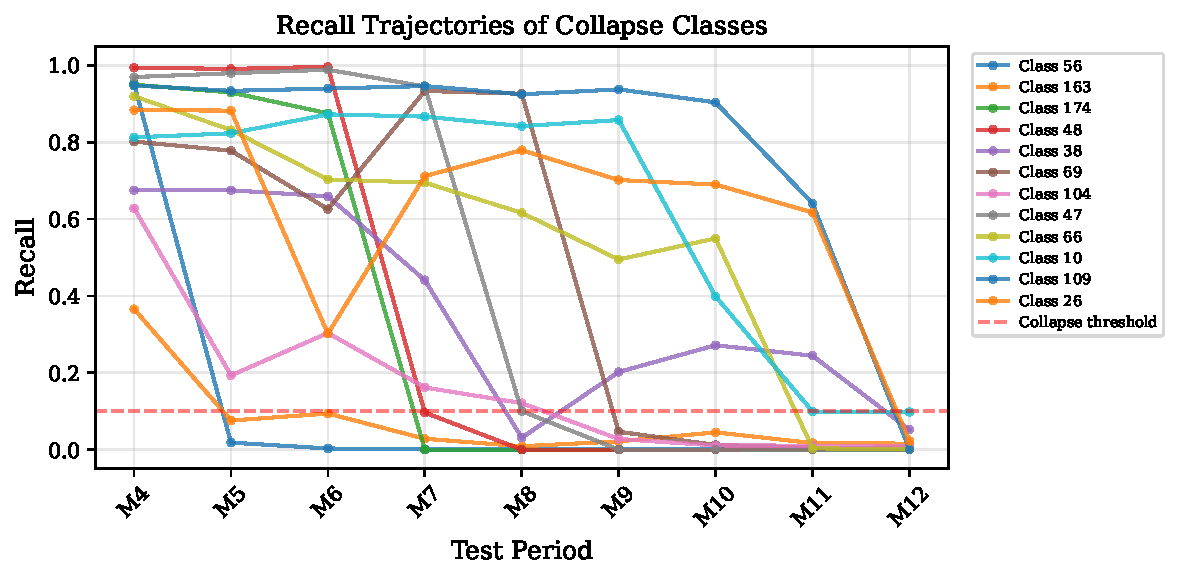
\includegraphics[width=\columnwidth]{fig_collapse_timeline.pdf}
\caption{Recall trajectories of 12 collapse classes on CESNET-TLS-Year22. Classes exhibit both abrupt collapse (\eg{}, class~56 at M5) and gradual decline (\eg{}, class~104 over M4--M12). By M12, all 12 classes fall below the 0.1 recall threshold (dashed line).}
\label{fig:collapse_timeline}
\end{figure}

Figure~\ref{fig:collapse_timeline} shows the recall trajectories of 12 classes that collapse below 0.1 recall by month~12.
The collapses follow two distinct temporal patterns:
\begin{itemize}
  \item \textbf{Abrupt collapse}: Recall drops sharply within one month (\eg{}, class~56 drops from 0.952 at M4 to 0.018 at M5).
  \item \textbf{Gradual collapse}: Recall decays over several months (\eg{}, class~104 declines from 0.629 at M4 to 0.028 at M9 and 0.010 by M12).
\end{itemize}

Crucially, these collapses are not random---each victim class has a \textit{primary absorber}: the dominant confusion target that receives the largest share of the victim's mispredictions.
Table~\ref{tab:absorber_pairs} lists the 12 collapse classes and their top absorbers, with confusion rates ranging from 13.9\% to 46.1\%.

\begin{table}[!htbp]
\centering
\caption{Absorber-collapse pairs at M-2022-12. Each collapsed class has a dominant confusion target (absorber). Confusion rate = fraction of victim samples predicted as the absorber.}
\label{tab:absorber_pairs}
\small
\begin{tabular}{@{}cccccc@{}}
\toprule
Victim & Absorber & Confusion & Victim & Pattern & First \\
Class  & Class    & Rate      & Recall & Type    & Collapse \\
\midrule
56  & 96  & 25.2\% & 0.000 & abrupt  & M5 \\
163 & 46  & 41.8\% & 0.015 & gradual & M5 \\
174 & 2   & 29.2\% & 0.000 & abrupt  & M7 \\
48  & 14  & 39.0\% & 0.001 & abrupt  & M7 \\
38  & 45  & 46.1\% & 0.052 & abrupt  & M8 \\
69  & 105 & 37.7\% & 0.005 & abrupt  & M9 \\
104 & 2   & 21.2\% & 0.010 & gradual & M9 \\
47  & 5   & 45.1\% & 0.000 & gradual & M11 \\
66  & 71  & 13.9\% & 0.001 & abrupt  & M11 \\
10  & 156 & 36.5\% & 0.098 & gradual & M11 \\
109 & 71  & 24.9\% & 0.000 & abrupt  & M12 \\
26  & 13  & 21.6\% & 0.022 & abrupt  & M12 \\
\bottomrule
\end{tabular}
\end{table}

\subsection{Two Empirical Signatures of Collapse}
\label{sec:mechanisms}

For descriptive analysis, we compare the Fisher discriminant ratio (inter-class distance divided by the sum of intra-class spreads) between victim--absorber pairs at M4 and M12. We group classes using heuristic thresholds on the relative change $\Delta J = (J_{\text{M12}} - J_{\text{M4}}) / J_{\text{M4}}$: a \textit{reduced-separability signature} when $\Delta J < -10\%$ and a \textit{boundary-mismatch signature} when $\Delta J > +20\%$. These groups are empirical signatures rather than identified causal mechanisms:

\begin{itemize}
  \item \textbf{Reduced-separability signature} (9 of 12 classes, including 56, 174, 104, and 109): The Fisher ratio decreases by 14--59\% (\eg{}, class~109$\to$71: 0.875 to 0.361), indicating reduced victim--absorber discriminability. The ratio alone does not distinguish centroid convergence from increased within-class spread.
  \item \textbf{Boundary-mismatch signature} (3 of 12 classes: 48, 69, and 10): Pairwise Fisher separation increases by 30--45\%, yet the frozen classifier still absorbs the victim. This is consistent with a mismatch between the representation and the learned decision boundary; shifts in other classes are one possible, untested explanation.
\end{itemize}

The two signatures motivate targeted boundary repair with broad class preservation. \ours{} combines target-label fine-tuning with all-class reference-period replay, but the analysis does not assign class-level causal mechanisms.

\begin{table}[!htbp]
\centering
\caption{Descriptive Fisher-ratio analysis for all 12 collapse classes. $J_{\text{M4}}$ and $J_{\text{M12}}$ denote victim--absorber Fisher ratios, and $\Delta J$ is the relative change. Threshold-defined groups are empirical signatures, not causal labels.}
\label{tab:fisher}
\scriptsize
\begin{tabular}{@{}r r l rr r r@{}}
\toprule
Victim & Abs. & Signature & $J_{\text{M4}}$ & $J_{\text{M12}}$ & $\Delta J$(\%) & Static \\
\midrule
\multicolumn{7}{@{}l}{\textit{Reduced separability ($\Delta J < -10\%$)}} \\
56  & 96  & red.\ sep. & 0.886 & 0.627 & $-$29 & 0.000 \\
174 & 2   & red.\ sep. & 0.635 & 0.326 & $-$49 & 0.000 \\
38  & 45  & red.\ sep. & 0.730 & 0.602 & $-$18 & 0.052 \\
163 & 46  & red.\ sep. & 0.308 & 0.265 & $-$14 & 0.016 \\
104 & 2   & red.\ sep. & 0.431 & 0.361 & $-$16 & 0.010 \\
47  & 5   & red.\ sep. & 0.781 & 0.513 & $-$34 & 0.000 \\
66  & 71  & red.\ sep. & 0.633 & 0.391 & $-$38 & 0.001 \\
109 & 71  & red.\ sep. & 0.875 & 0.361 & $-$59 & 0.000 \\
26  & 13  & red.\ sep. & 0.367 & 0.188 & $-$49 & 0.022 \\
\midrule
\multicolumn{7}{@{}l}{\textit{Boundary mismatch ($\Delta J > +20\%$)}} \\
48  & 14  & bnd.\ mismatch & 0.561 & 0.730 & $+$30 & 0.001 \\
69  & 105 & bnd.\ mismatch & 0.293 & 0.426 & $+$45 & 0.005 \\
10  & 156 & bnd.\ mismatch & 0.435 & 0.567 & $+$30 & 0.098 \\
\bottomrule
\end{tabular}
\end{table}

Table~\ref{tab:fisher} quantifies the Fisher discriminant ratio trajectory for all 12 collapse classes.
Reduced-separability classes (9 of 12) exhibit a mean $\Delta J = -34\%$, indicating lower victim--absorber discriminability at M12.
Boundary-mismatch classes (3 of 12) show the opposite ($\Delta J \approx +35\%$): pairwise separation increases despite continued collapse, which is consistent with a frozen-boundary mismatch but does not identify its cause.

\begin{figure}[!htbp]
\centering
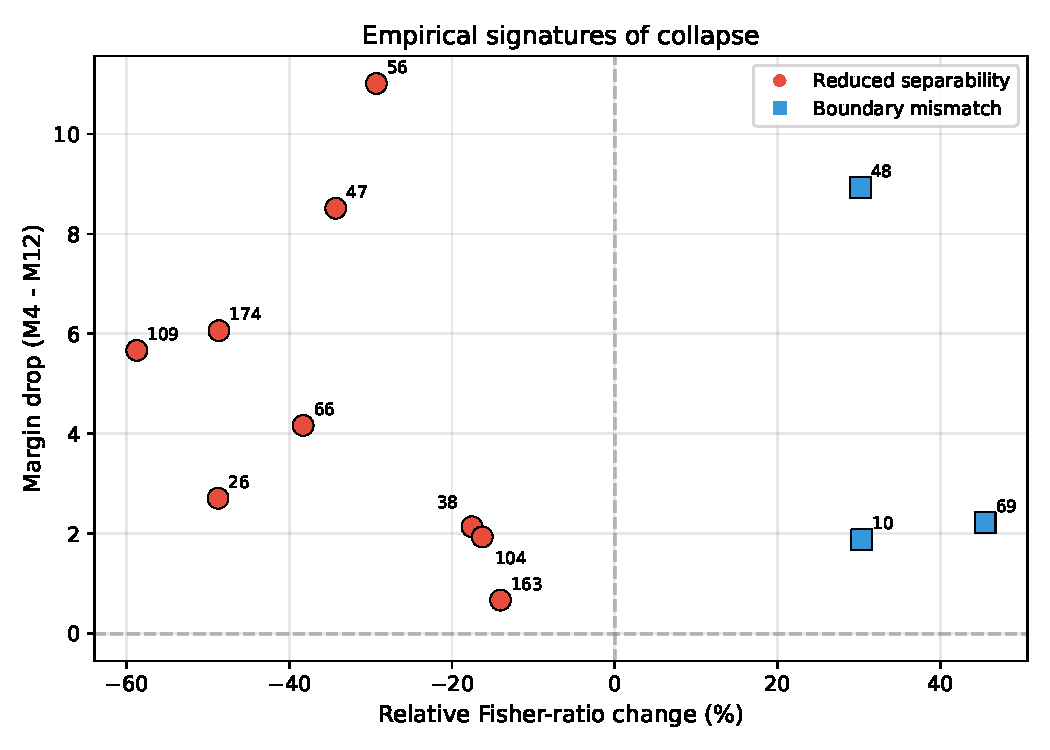
\includegraphics[width=\columnwidth]{drift_scatter.pdf}
\caption{Scatter plot of the two descriptive signatures for all 12 collapse classes. The x-axis shows relative Fisher-ratio change ($\Delta J$) from M4 to M12; the y-axis shows margin drop (M4 margin $-$ M12 margin). Colors reproduce the threshold-defined groups. All classes show positive margin drops (0.67--11.01), and 11 of 12 exceed 1.5, consistent with reduced logit separation. Replotted from archived numeric records using a Codex-assisted Matplotlib script; the plotted values are unchanged.}
\label{fig:drift_scatter}
\end{figure}
\FloatBarrier

Figure~\ref{fig:drift_scatter} positions each collapse class by its Fisher-ratio change and margin drop.
The x-axis separation visualizes the threshold-defined grouping by construction and is not independent validation; the overlapping margin drops show that margin alone does not distinguish the two signatures.

\subsection{Why General TTA Methods Fail}
\label{sec:tta_eval}

We evaluate five TTA methods from computer vision on the same setup: Tent~\cite{wang2021tent}, EATA~\cite{niu2022eata}, SAR~\cite{niu2023sar}, CoTTA~\cite{wang2022cotta}, and NOTE~\cite{gong2022note}.
These are traffic-adapted implementations for 1D packet-sequence inputs, with necessary simplifications: EATA uses uniform Fisher importance (rather than per-sample Fisher computed from a held-out set), CoTTA uses Gaussian noise augmentation (as no standard augmentation pipeline exists for packet sequences), and NOTE uses a simplified prediction-balanced buffer without Instance-Aware BatchNorm.
Table~\ref{tab:tta} reports M12 results.

\begin{table}[!htbp]
\centering
\caption{TTA baselines on CESNET-TLS-Year22 at M-2022-12 (traffic-adapted implementations, no labels). None of the tested variants repair collapse classes under our implementations.}
\label{tab:tta}
\small
\begin{tabular}{@{}l ccc@{}}
\toprule
Method & Macro-F1 & Collapse F1 & Stable F1 \\
\midrule
Static      & 0.629 & 0.028 & 0.903 \\
Tent        & 0.631 & 0.026 & 0.903 \\
EATA        & 0.629 & 0.028 & 0.903 \\
SAR         & 0.629 & 0.026 & 0.901 \\
CoTTA       & 0.630 & 0.027 & 0.903 \\
NOTE        & 0.630 & 0.027 & 0.902 \\
\bottomrule
\end{tabular}
\end{table}

These simplifications may underestimate the methods' potential; however, the near-zero collapse F1 across all tested variants---including Tent and SAR, which require no simplification---is consistent with a mismatch between confidence-based unsupervised adaptation and confident absorber--victim errors.
When an absorber class confidently captures a victim's predictions, entropy is \textit{low} (the model is confidently wrong), so entropy-based adaptation sees no signal to correct.
This negative result motivates the shift from unsupervised adaptation to label-efficient targeted repair.

To assess learning-rate sensitivity, we sweep five learning rates from $10^{-5}$ to $10^{-3}$ (5 configurations per method).
The best collapse F1 across all configurations remains below 0.031 for every method (NOTE: 0.030, EATA: 0.028, CoTTA: 0.027, SAR: 0.027, Tent: 0.026), showing limited sensitivity to learning-rate choice over the tested range.
Higher learning rates cause Tent to catastrophically degrade (macro-F1 drops from 0.63 to 0.21 at learning rate $10^{-3}$).

% ============================================================
\section{Method: Collapse-Aware Repair}
\label{sec:method}

\ours{} is a label-efficient repair framework comprising three stages: (1)~unsupervised monitoring of per-class health, (2)~active sample selection, and (3)~head fine-tuning with all-class replay and knowledge distillation.
Algorithm~\ref{alg:care} summarizes the procedure.

Figure~\ref{fig:care_workflow} gives the proposed operator-reviewed workflow.

\begin{figure}[H]
\centering
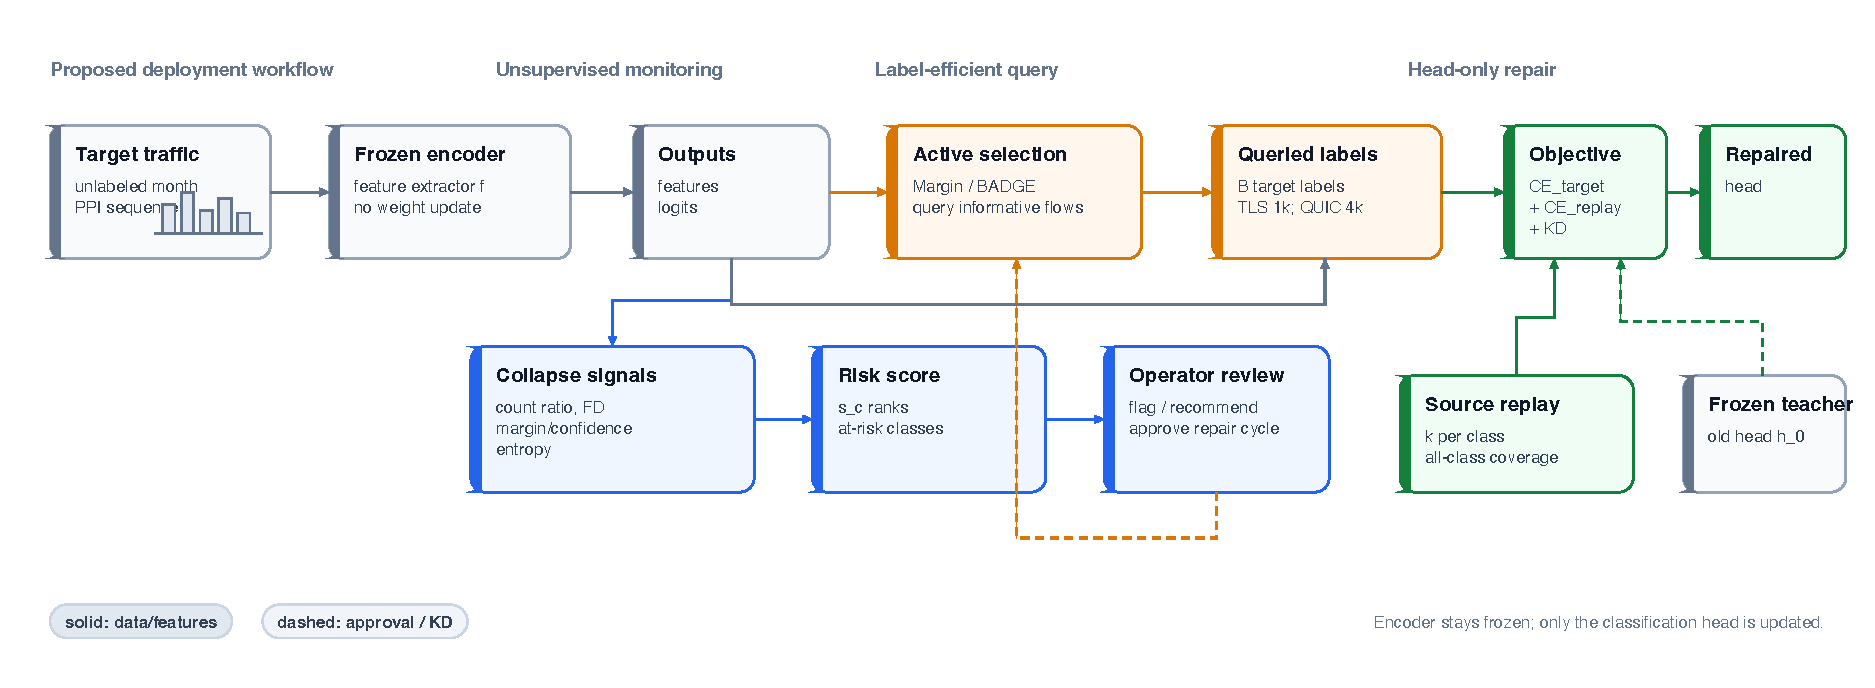
\includegraphics[width=\textwidth]{fig_care_workflow_v4.pdf}
\caption{Proposed operator-reviewed \ours{} workflow. A frozen encoder produces target-period logits and features. Monitoring ranks class-level risk and flags classes for operator review; only an approved repair cycle proceeds to active label selection and offline head-only repair with all-class reference-period replay and knowledge distillation.}
\label{fig:care_workflow}
\end{figure}
\FloatBarrier

\subsection{Unsupervised Collapse Detection and Monitoring}
\label{sec:unsup_detect}

We propose a multi-signal collapse risk score computed entirely from model predictions on unlabeled data.
For each class $c$, we compare predictions between a reference period and the target period across five signals, all computed on samples \textit{predicted} as class $c$ (no true labels required):
\begin{enumerate}
  \item \textbf{Prediction count ratio}: $r_c = (n_c^{\text{tgt}}/N^{\text{tgt}}) / (n_c^{\text{ref}}/N^{\text{ref}})$. Collapsed classes lose predictions ($r_c \ll 1$).
  \item \textbf{Fr\'{e}chet Distance (FD)}: Feature distribution shift between periods for the predicted class region.
  \item \textbf{Margin drop}: Decrease in mean prediction margin (top-2 logit gap).
  \item \textbf{Confidence drop}: Decrease in mean prediction confidence.
  \item \textbf{Entropy rise}: Increase in mean prediction entropy.
\end{enumerate}

The collapse risk score combines these signals:
\begin{equation}
  s_c = w_1 \cdot \max(0, 1{-}r_c) + w_2 \cdot \tilde{d}_c + w_3 \cdot \tilde{m}_c + w_4 \cdot \tilde{f}_c + w_5 \cdot \tilde{e}_c
\end{equation}
where $\tilde{d}_c$, $\tilde{m}_c$, $\tilde{f}_c$, $\tilde{e}_c$ denote the median-absolute-deviation (MAD)-normalized FD, margin drop, confidence drop, and entropy rise for class $c$, and $w = (0.40, 0.20, 0.15, 0.15, 0.10)$.
Weights were set as a fixed heuristic based on signal informativeness (count drop is the strongest single indicator), without access to target-period labels; labels are used only retrospectively to report detection precision and recall.
A sensitivity analysis (\S\ref{sec:detection_eval}) comparing manual, equal, and historically calibrated weights shows limited variation across the three tested settings (detection F1 0.563--0.625 on M12).
In the reported diagnostic, candidates must satisfy $s_c>0.12$, after which at most the 20 highest-risk classes are retained.
This is an evaluation operating point for operator review, not a validated automatic retraining gate.

This module serves two intended roles in the proposed workflow:
\begin{itemize}
  \item \textbf{Monitoring}: It flags classes at risk of degradation for operator investigation.
  \item \textbf{Alerting}: Per-class risk scores inform \textit{when} repair should be considered, without requiring labeled data to detect drift.
\end{itemize}
Importantly, the detection module does \textit{not} guide replay class selection---all-class replay is the default (\S\ref{sec:replay_ablation}).

\subsection{Active Sample Selection}
\label{sec:sample_select}

From the target period, we select a budget $B$ of samples for labeling.
\textit{Margin sampling} selects globally low-margin samples, which may include absorber--victim boundaries.
\textit{BADGE}~\cite{ash2020badge} selects diverse uncertain samples via gradient embeddings and achieves higher mean performance with greater algorithmic complexity than margin.
Given precomputed logits and features, Margin ranks one scalar top-two gap per target instance. Our BADGE implementation forms top-three-class gradient embeddings, applies 50-dimensional principal component analysis, and performs $B$ k-means++ seeding steps; its iterative seeding is therefore substantially more expensive than Margin's global score sort. Table~\ref{tab:matched_holdout} reports program-level rather than selector-only wall time.

\subsection{Head Fine-Tuning with All-Class Reference-Period Replay}
\label{sec:ft_replay}

We precompute frozen features $z=f(x)$ and fine-tune only $h_\theta$ using selected target features plus $k{=}5$ labeled reference feature exemplars per class (890 total). Let $D_{\text{train}}^z$ be the training multiset containing $\rho$ copies of each queried target feature and one copy of each reference exemplar; the default target repeat is $\rho{=}2$:
\begin{equation}
  \mathcal{L}_{\text{ft}} = \frac{1}{|D_{\text{train}}^z|} \sum_{(z,y)\in D_{\text{train}}^z} \ell_{\text{CE}}(h_\theta(z), y)
\end{equation}
where $\ell_{\text{CE}}$ is cross-entropy loss and $|D_{\text{train}}^z|=\rho B+890$. Thus the default $B{=}1{,}000$ update uses 2{,}890 training feature entries but only 1{,}000 unique newly labeled target samples.
All-class replay covers all 178 classes and performs better than targeted replay in the evaluated strategy study (\S\ref{sec:replay_ablation}).

\subsection{Knowledge Distillation}
\label{sec:distill}

On replay feature exemplars, we add a KL-divergence loss~\cite{hinton2015distilling} between the updated head $h_\theta$ and original head $h_{\theta_0}$:
\begin{equation}
  \mathcal{L}_{\text{KD}} = \frac{T^2}{|D_{\text{replay}}^z|} \!\sum_{z \in D_{\text{replay}}^z} D_{\text{KL}}\!\!\left(\sigma\!\!\left(\frac{h_{\theta_0}(z)}{T}\right) \!\Big\|\! \sigma\!\!\left(\frac{h_\theta(z)}{T}\right)\!\right)
\end{equation}
where $T$ is the temperature and $\sigma$ is softmax. The $T^2$ factor matches the implementation. Each update independently samples a reference minibatch with replacement for distillation.
Distillation is applied only on replay features because the teacher's reference-period predictions represent its source behavior.
On target samples, the teacher's predictions may already reflect absorber-collapse errors, making them unsuitable as distillation targets.

\subsection{Combined Objective and Algorithm}

The full training loss is:
\begin{equation}
  \mathcal{L} = \mathcal{L}_{\text{ft}} + \lambda_{\text{KD}} \cdot \mathcal{L}_{\text{KD}}
\end{equation}

\begin{algorithm}[t]
\caption{\ours{}: Collapse-Aware Repair}
\label{alg:care}
\begin{algorithmic}[1]
\REQUIRE Source model $f, h_{\theta_0}$; labeled reference features and reference predictions; unlabeled target data $D_{\text{tgt}}$; budget $B$; repeat $\rho$; epochs $E$
\STATE \textbf{Monitor:} Compute per-class risk scores $s_c$ (\S\ref{sec:unsup_detect}) from unlabeled predictions
\STATE \textbf{Alert:} Flag risk for operator review; proceed only after operator approval
\STATE Compute features and logits for $D_{\text{tgt}}$
\STATE Select $B$ samples via margin or BADGE; query labels $\to D_{\text{tgt}}^z$
\STATE Sample $D_{\text{replay}}^z$: $k{=}5$ frozen features from labeled reference-period data for all 178 classes
\STATE Build $D_{\text{train}}^z$ with $\rho$ target copies and one reference copy
\STATE Initialize $h_\theta \leftarrow h_{\theta_0}$
\FOR{epoch $= 1, \ldots, E$}
  \FOR{minibatch in a shuffled pass over $D_{\text{train}}^z$}
    \STATE Independently sample a reference minibatch for KD
    \STATE $\mathcal{L} \leftarrow \mathcal{L}_{\text{ft}} + \lambda_{\text{KD}} \cdot \mathcal{L}_{\text{KD}}$
    \STATE Update $\theta$ via AdamW on $\mathcal{L}$
  \ENDFOR
\ENDFOR
\RETURN Updated classifier $h_\theta$
\end{algorithmic}
\end{algorithm}


% ============================================================
\section{Experiments}
\label{sec:experiments}

This section evaluates \ours{} from four complementary perspectives: overall repair performance and baseline comparisons, internal mechanisms and design choices, generalization and robustness, and diagnostic detection quality. We first describe the datasets, evaluation protocols, metrics, and implementation settings.

\subsection{Experimental Setup}
\label{sec:exp_setup}

Datasets.
We use CESNET-TLS-Year22~\cite{hynek2024cesnet} (178 classes, 12 months, TLS traffic) as the primary benchmark and CESNET-QUICEXT-25 XS~\cite{cesnetquicext25,mucke2025waiting} as a supporting cross-protocol stress test.
Our experiments use monthly DataZoo partitions for both datasets and evaluate drift at month-level granularity; they do not replay flows in timestamp order.
For TLS-Year22, we train on M-2022-3 and evaluate at M7, M9, M11, and M12.
For QUICEXT-25, we train on M-2024-6 and evaluate on M-2025-5.

Dataset-specific collection change.
CESNET-TLS-Year22 has a known distribution shift at week~10 due to a flow exporter update~\cite{hynek2024cesnet}.
The change is shared by all methods evaluated on the same chronological split, but it remains a dataset-specific source of shift that limits causal attribution to application evolution alone.

Baselines.
We compare five categories:
(1)~\textit{Unsupervised TTA} (0 labels): Tent~\cite{wang2021tent}, EATA~\cite{niu2022eata}, SAR~\cite{niu2023sar}, CoTTA~\cite{wang2022cotta}, NOTE~\cite{gong2022note}.
(2)~\textit{Self-evolving pseudo-label adaptation} (0 human labels): a Chen-inspired full-model baseline~\cite{chen2025selfevolving} (\S\ref{sec:matched_holdout}).
(3)~\textit{Standard active learning} (1{,}000 labels + \ours{} components): entropy, coreset~\cite{sener2018coreset}, random.
(4)~\textit{Continual learning / drift adaptation} (1{,}000 labels): MEMENTO~\cite{cerasuolo2024memento}, ILETC~\cite{zhu2023iletc}, CADE~\cite{yang2021cade}, expanded head (\S\ref{sec:cl_baselines}).
(5)~\textit{\ours{} configurations} (1{,}000 labels): margin and BADGE~\cite{ash2020badge} with all-class replay.

Evaluation protocol.
Under the main \textit{strict} protocol, active methods query from the full target pool and the selected samples are excluded before computing metrics. The separate matched-holdout protocol first reserves a fixed seed-wise 20\% test subset, uses the remaining 80\% only for adaptation, and evaluates the predefined 12 M12 collapse classes on the untouched holdout.
Static and TTA rows are single-checkpoint evaluations.
Main active-learning and \ours{} rows use the same fixed source checkpoint and report mean $\pm$ sample standard deviation over five run seeds, which control stochastic selection where applicable, replay sampling, and head-update shuffling; they are not independently trained source encoders.
Multi-period, prototype, and architecture studies use three run seeds as noted.
The separate retraining audit uses three source-model training seeds and three repair seeds per model.

Metrics.
(1)~Overall macro-F1 (all 178 classes);
(2)~collapse-class macro-F1 (12 classes with recall ${<}0.1$ in the static model at M12);
(3)~stable-class macro-F1, the unweighted mean of global per-class F1 over a fixed 20-class post-hoc diagnostic set selected by the smallest absolute M4-to-M12 F1 change among classes with at least 100 M12 instances and nonzero M4 support\footnote{Class IDs: 8, 15, 44, 57, 59, 62, 64, 76, 94, 98, 99, 107, 113, 119, 128, 130, 131, 132, 144, and 145.}; this endpoint-defined set measures preservation and does not imply high recall in every intervening month;
(4)~number of classes in the predefined collapse group that remain below 0.1 recall (12 classes for TLS and three for the QUIC stress test); this is not a count of newly collapsed classes outside that group;
(5)~per-class \textit{recovery status}: recovered ($R{\geq}0.30$), partial ($0.05{\leq}R{<}0.30$), or failed ($R{<}0.05$). We assign these recovery statuses from each class's mean recall across repair seeds and report counts separately for each fixed selector.
Tables abbreviate the last three aggregate metrics as Col.\ F1, Stb.\ F1, and \#Col., respectively.

\ours{} configuration.
Budget $B{=}1{,}000$, all-class replay with $k{=}5$ per class (890 features), target repeat factor 2, $\lambda_{\text{KD}}{=}0.5$, $T{=}2.0$, head fine-tuning learning rate $10^{-3}$, and 30 epochs. The default monitoring/replay reference is M4; the classifier is trained on M3.

Collapse-definition sensitivity.
Across all tested thresholds and support settings, \ours{} preserves substantial collapse-class recovery: the identified set varies from 10 to 13 classes, yet the collapse-F1 gain remains $\Delta{=}0.208$--$0.246$. Support thresholds of 50 and 100 yield identical results, while $s{=}200$ removes only the borderline class 38 at $\tau{=}0.10$ and $0.15$. These results show that the main conclusion is robust to the tested collapse definitions; broader threshold ranges remain for future validation.

\subsection{Overall Performance}
\label{sec:main_results}

Overall performance is assessed in four stages: the primary strict query-excluded evaluation at M12, a seed-matched holdout comparison with self-evolving adaptation, comparisons with continual-learning baselines, and performance across drift periods.

\subsubsection{Primary Results under Strict Query-Excluded Evaluation}
\label{sec:primary_results}

Table~\ref{tab:main_results} presents the main comparison at M-2022-12 (nine months after training).

\begin{table}[!htbp]
\centering
\caption{Main results on CESNET-TLS-Year22 at M-2022-12. Static/TTA rows are single-checkpoint evaluations without labels. Active rows use $B{=}1{,}000$ labels, M4 all-class replay ($k{=}5$, 890 features), KD ($\lambda{=}0.5$), strict query exclusion, and five seeds.}
\label{tab:main_results}
\scriptsize
\setlength{\tabcolsep}{3pt}
\begin{tabular}{@{}l cccc@{}}
\toprule
Method & Macro & Col.\ F1 & Stb.\ F1 & \#Col \\
\midrule
\multicolumn{5}{l}{\textit{No labeled target data:}} \\
Static          & 0.629 & 0.028 & 0.903 & 12 \\
Tent            & 0.631 & 0.026 & 0.903 & 12 \\
EATA            & 0.629 & 0.028 & 0.903 & 12 \\
SAR             & 0.629 & 0.026 & 0.901 & 11 \\
CoTTA           & 0.630 & 0.027 & 0.903 & 12 \\
NOTE            & 0.630 & 0.027 & 0.902 & 12 \\
\midrule
\multicolumn{5}{l}{\textit{Active ($B$=1000, all-class replay+KD, 5 seeds):}} \\
Entropy         & 0.628$\pm$0.004 & 0.078$\pm$0.015 & 0.887$\pm$0.004 & 10.2 \\
Coreset         & 0.633$\pm$0.005 & 0.116$\pm$0.042 & 0.886$\pm$0.007 & 8.8 \\
Random          & 0.668$\pm$0.004 & 0.188$\pm$0.024 & 0.892$\pm$0.006 & 8.2 \\
\ours{}-Margin  & 0.686$\pm$0.001 & 0.256$\pm$0.009 & 0.892$\pm$0.003 & 5.8 \\
\textbf{\ours{}-BADGE} & \textbf{0.700$\pm$0.003} & \textbf{0.332$\pm$0.040} & \textbf{0.894$\pm$0.004} & \textbf{4.0} \\
\bottomrule
\end{tabular}
\end{table}

CARE-BADGE has the highest mean macro-F1 and collapse-class F1 among the repair rows in Table~\ref{tab:main_results}, raising macro-F1 to $0.700{\pm}0.003$ and collapse-class F1 to $0.332{\pm}0.040$ while retaining stable-class F1 of 0.894. CARE-Margin provides a lower-cost operating point with macro-F1 of $0.686{\pm}0.001$ and collapse F1 of $0.256{\pm}0.009$. By contrast, the five tested label-free TTA variants leave collapse F1 below 0.031, and generic entropy and coreset selectors trail random, Margin, and BADGE under the same replay-and-distillation pipeline. These results support the value of verified target labels and appropriate query selection for collapse repair.

Selector-level statistical comparison.
\label{sec:significance}
Paired $t$-tests on the strict main experiment provide exploratory evidence for Margin over Random (macro-F1 $p{=}0.00075$; collapse F1 $p{=}0.00262$) and BADGE over Margin (macro-F1 $p{=}0.00112$; collapse F1 $p{=}0.0177$).
The corresponding exact Wilcoxon signed-rank tests are not significant at $n{=}5$ (minimum attainable two-sided $p{=}0.0625$), so these rankings are reported with effect sizes and seed-wise variance rather than treated as definitive.

\subsubsection{Seed-Matched Holdout Comparison with Self-Evolving Adaptation}
\label{sec:matched_holdout}

For a direct comparison with self-evolving adaptation, we conducted a separate seed-matched experiment on the same 1{,}323{,}229-instance M12 target pool. This is a Chen-inspired pseudo-label baseline, not an exact reproduction of \citet{chen2025selfevolving}.
Starting from the same source checkpoint (\texttt{tls22\_cnn/best\_model.pt}), each seed uses \texttt{RandomState(seed+42)} to split the target pool into a 1{,}058{,}584-instance adaptation subset (80\%) and a 264{,}645-instance untouched holdout (20\%). Adaptation samples whose maximum softmax confidence meets or exceeds $p\in\{0.90,0.95,0.99,0.997\}$ receive argmax pseudo-labels. We update the encoder and head with AdamW (learning rate 0.0025, weight decay $10^{-4}$, batch size 500, 50 epochs), without human target labels, replay, or KD.
All values in Table~\ref{tab:matched_holdout} are computed exclusively on the untouched holdout. We show the paper-aligned $p{\geq}0.997$ row and the post-hoc setting with the highest overall macro-F1, $p{\geq}0.90$; the latter was not selected on an independent validation set and should not be read as a preregistered operating point.

\begin{table}[!htbp]
\centering
\caption{Seed-matched 20\% holdout comparison at M12 (mean $\pm$ sample standard deviation over 5 seeds). Human labels count unique queried target labels; pseudo-labels are the mean high-confidence target samples used for our Chen-style full-model fine-tuning. Program wall time is measured on one NVIDIA L20 under each method's final configuration; dashes denote configurations not included in the timing run.}
\label{tab:matched_holdout}
\scriptsize
\resizebox{\textwidth}{!}{%
\begin{tabular}{@{}l rr ccccc@{}}
\toprule
Method & Human & Pseudo & Macro F1 & Collapse F1 & Stable F1 & \#Col. & Wall (s) \\
\midrule
Static & 0 & 0 & $0.6308{\pm}0.0020$ & $0.0313{\pm}0.0055$ & $0.9019{\pm}0.0015$ & 11.8 & -- \\
Chen-style ($p{\geq}0.997$) & 0 & 298.8K & $0.5050{\pm}0.0097$ & $0.0008{\pm}0.0018$ & $0.8063{\pm}0.0208$ & 12.0 & $80.0{\pm}1.0$ \\
Chen-style ($p{\geq}0.90$, sensitivity) & 0 & 628.7K & $0.6140{\pm}0.0058$ & $0.0136{\pm}0.0035$ & $0.8887{\pm}0.0080$ & 12.0 & $136.4{\pm}0.5$ \\
\midrule
\ours{}-Entropy & 1{,}000 & 0 & $0.6316{\pm}0.0025$ & $0.0797{\pm}0.0097$ & $0.8863{\pm}0.0039$ & 10.0 & -- \\
\ours{}-Random & 1{,}000 & 0 & $0.6722{\pm}0.0021$ & $0.2246{\pm}0.0370$ & $0.8934{\pm}0.0039$ & 7.0 & -- \\
\ours{}-Margin & 1{,}000 & 0 & $0.6885{\pm}0.0022$ & $0.2835{\pm}0.0185$ & $0.8932{\pm}0.0047$ & \textbf{4.6} & $48.5{\pm}0.8$ \\
\ours{}-BADGE & 1{,}000 & 0 & $\mathbf{0.7008{\pm}0.0068}$ & $\mathbf{0.3099{\pm}0.0473}$ & $\mathbf{0.9004{\pm}0.0042}$ & 4.8 & $166.6{\pm}8.2$ \\
\bottomrule
\end{tabular}}
\end{table}

On the common untouched holdouts, \ours{}-BADGE achieves the highest mean macro-F1 (0.701) and collapse F1 (0.310). The best-macro Chen-style sensitivity setting reaches 0.614 and 0.014, respectively, and leaves all 12 classes below the collapse threshold. This establishes a large repair advantage on identical seed-wise holdouts, although the methods use different supervision and update budgets: the Chen-style implementation uses high-confidence pseudo-labels and full-model fine-tuning, whereas \ours{} uses 1{,}000 verified target labels, 890 reference features, and head-only repair. Within \ours{}, Margin exceeds Random after Holm correction; BADGE has higher mean macro-F1 and collapse F1 than Margin, but five seeds do not resolve that selector-level difference.

\subsubsection{Comparison with Continual Learning Baselines}
\label{sec:cl_baselines}

To situate \ours{} against continual-learning and drift-adaptation methods, we adapt four representative approaches to our collapse-repair setting (Table~\ref{tab:cl_baselines}).
All labeled methods use $B{=}1{,}000$, strict query exclusion, and five seeds. Except for selector-specific CADE-score and \ours{}-BADGE rows, labeled baselines use the same Margin-selected batch. Except for MEMENTO (which fine-tunes the full model), all methods share the same frozen encoder and differ in how the classification head is updated or what replay data is used.

\begin{itemize}
  \item \textbf{MEMENTO}~\cite{cerasuolo2024memento}: Full-model fine-tuning (encoder + head) with KD on all-class replay. MEMENTO's output rectification reduces to a no-op when replaying all classes, so we report the core mechanism only.
  \item \textbf{ILETC}~\cite{zhu2023iletc}: A conditional Wasserstein generative adversarial network with gradient penalty (WGAN-GP) generates synthetic replay features per class; the head is fine-tuned on target labels + generated replay without knowledge distillation.
  \item \textbf{CADE-score}~\cite{yang2021cade}: A contrastive autoencoder computes per-sample drift scores; the top-$B$ highest-scoring samples are selected for labeling instead of margin sampling. Repair uses the same head fine-tuning + replay + KD pipeline as \ours{}.
  \item \textbf{Expanded head} (inspired by PRIME~\cite{prime2025}): The single-layer head (Linear(256, $C$)) is replaced by a two-layer head (Linear(256, 512)$\to$rectified linear unit (ReLU)$\to$Linear(512, $C$)), initialized via a dual-channel decomposition that reproduces the original output before fine-tuning. PRIME targets new classes; we evaluate capacity expansion for fixed-class repair.
\end{itemize}

\begin{table}[!htbp]
\centering
\caption{Continual-learning and drift-adaptation baselines at M-2022-12 ($B{=}1{,}000$, strict eval, 5 seeds). CADE-score and CARE-BADGE use their named selectors; other labeled rows use Margin. CARE rows are reproduced from Table~\ref{tab:main_results}.}
\label{tab:cl_baselines}
\scriptsize
\setlength{\tabcolsep}{3pt}
\begin{tabular}{@{}l cccc@{}}
\toprule
Method & Macro & Col.\ F1 & Stb.\ F1 & \#Col \\
\midrule
Static & 0.629 & 0.028 & \textbf{0.903} & 12.0 \\
\midrule
\multicolumn{5}{l}{\textit{CL / drift baselines (same label budget):}} \\
CADE-score~\cite{yang2021cade}     & 0.637$\pm$0.004 & 0.118$\pm$0.015 & 0.889$\pm$0.003 & 9.0 \\
ILETC-GAN~\cite{zhu2023iletc}     & 0.650$\pm$0.004 & 0.219$\pm$0.010 & 0.851$\pm$0.009 & 5.4 \\
ILETC-real                         & 0.659$\pm$0.003 & 0.236$\pm$0.010 & 0.854$\pm$0.016 & 4.8 \\
Expanded head                      & 0.673$\pm$0.003 & 0.307$\pm$0.005 & 0.871$\pm$0.008 & 4.8 \\
MEMENTO~\cite{cerasuolo2024memento}& 0.678$\pm$0.002 & 0.255$\pm$0.005 & 0.892$\pm$0.004 & 6.0 \\
\midrule
\ours{}-Margin & 0.686$\pm$0.001 & 0.256$\pm$0.009 & 0.892$\pm$0.003 & 5.8 \\
\textbf{\ours{}-BADGE} & \textbf{0.700$\pm$0.003} & \textbf{0.332$\pm$0.040} & 0.894$\pm$0.004 & \textbf{4.0} \\
\bottomrule
\end{tabular}
\end{table}

Three findings emerge:
\begin{itemize}
  \item \textbf{Full-model fine-tuning does not improve this operating point.} Under this 1{,}000-label budget and implementation, MEMENTO achieves comparable collapse F1 to \ours{}-Margin (0.255 vs.\ 0.256) but lower macro-F1 (0.678 vs.\ 0.686), supporting the head-only design for the evaluated setting.
  \item \textbf{Under this implementation, GAN-generated replay trails real replay.} ILETC-GAN underperforms ILETC-real on macro-F1 (0.650 vs.\ 0.659) and collapse F1 (0.219 vs.\ 0.236), and both trail \ours{}-Margin. The experiment does not isolate why. Their larger stable-class degradation (0.851--0.854 vs.\ 0.892) is consistent with omitting knowledge distillation, although this attribution is not isolated.
  \item \textbf{Capacity expansion helps collapse but hurts stability.} The expanded head reaches 0.307 collapse F1 but 0.871 stable-class F1 and 0.673 macro-F1. \ours{}-BADGE has higher mean macro-F1 and collapse F1 among the evaluated repair rows, limiting the decrease in stable-class F1 relative to the static baseline to 0.009.
\end{itemize}

CADE-score has the lowest collapse F1 among the repair rows in Table~\ref{tab:cl_baselines} (0.118); this result is consistent with the hypothesis that anomaly-oriented scores need not select boundary-informative samples, but the mechanism was not isolated. Overall, \ours{}-BADGE has the highest mean macro-F1 and collapse F1 among the evaluated repair methods.

\subsubsection{Multi-Period Generalization}
\label{sec:multi_period}

Table~\ref{tab:multiperiod} shows \ours{}'s effectiveness across four time points with increasing drift severity.

\begin{table}[!htbp]
\centering
\caption{Multi-period results (Margin, $B$=1000, all-class replay $k{=}5$, 3 seeds). The fixed collapse set is the 12 classes identified by the M12 static model.}
\label{tab:multiperiod}
\scriptsize
\setlength{\tabcolsep}{3pt}
\begin{tabular}{@{}l cc cc c@{}}
\toprule
& \multicolumn{2}{c}{Static} & \multicolumn{2}{c}{\ours{}} & \\
\cmidrule(lr){2-3} \cmidrule(lr){4-5}
Period & Macro & Col. & Macro & Col. & $\Delta$ Macro \\
\midrule
M7 (light)   & 0.740 & 0.503 & 0.776$\pm$0.003 & 0.633$\pm$0.028 & +0.036 \\
M9 (medium)  & 0.691 & 0.280 & 0.739$\pm$0.003 & 0.392$\pm$0.005 & +0.048 \\
M11 (heavy)  & 0.649 & 0.145 & 0.708$\pm$0.002 & 0.408$\pm$0.016 & +0.060 \\
M12 (severe) & 0.629 & 0.028 & 0.686$\pm$0.002 & 0.255$\pm$0.012 & +0.057 \\
\bottomrule
\end{tabular}
\end{table}

\ours{} improves both macro-F1 and collapse F1 at every evaluated drift level. Macro-F1 gains range from +0.036 at M7 to +0.060 at M11, while collapse F1 reaches 0.633 at M7 and remains 0.255 even under severe M12 drift. This consistent pattern demonstrates robustness across drift severity and indicates that earlier maintenance can offer stronger recoverability; sequential interventions remain to be tested.

\subsection{Internal Mechanism Analysis}
\label{sec:mechanism_analysis}

This subsection analyzes how the main components and design choices contribute to repair, covering component variants, sample-selection strategies, and replay strategies.

\subsubsection{Component-Variant Study}
\label{sec:ablation}

Table~\ref{tab:ablation} compares seven implementation variants, summarized in Figure~\ref{fig:ablation_bar}. All use Margin selection, strict evaluation, and five seeds, but the study is not fully factorial: FT-only/FT+KD use target repeat 1, FT+Rpl/Full CARE use repeat 2, and FT+KD uses 150 targeted replay features rather than 890 all-class features. The rows compare evaluated bundles rather than isolating single-component effects.

\begin{table}[!htbp]
\centering
\caption{Component variants at M12 (Margin, strict evaluation, 5 seeds). Targeted-150 contains stable+absorber features; All-890 contains five features per class. FT, Rpl, KD, and Rep. denote fine-tuning, replay, knowledge distillation, and target repeat.}
\label{tab:ablation}
\scriptsize
\setlength{\tabcolsep}{2pt}
\resizebox{\textwidth}{!}{%
\begin{tabular}{@{}l c l c c ccc c@{}}
\toprule
Config. & Target $B$ & Replay & KD & Rep. & Macro & Col.\ F1 & Stb.\ F1 & \#Col \\
\midrule
Static & 0 & None & -- & -- & 0.629 & 0.028 & \textbf{0.903} & 12 \\
\midrule
Replay only & 0 & All-890 & -- & -- & 0.563$\pm$0.007 & 0.044$\pm$0.019 & 0.816$\pm$0.026 & 10.2 \\
Rpl+KD & 0 & All-890 & \checkmark & -- & 0.618$\pm$0.005 & 0.039$\pm$0.016 & 0.888$\pm$0.009 & 10.8 \\
\midrule
FT only & 1000 & None & -- & 1 & 0.638$\pm$0.000 & 0.134$\pm$0.001 & 0.839$\pm$0.001 & 7.0 \\
FT+KD & 1000 & Targeted-150 & \checkmark & 1 & 0.670$\pm$0.000 & 0.152$\pm$0.007 & 0.887$\pm$0.004 & 7.8 \\
FT+Rpl & 1000 & All-890 & -- & 2 & 0.659$\pm$0.003 & 0.236$\pm$0.010 & 0.854$\pm$0.016 & 4.8 \\
\textbf{Full \ours{}} & 1000 & All-890 & \checkmark & 2 & \textbf{0.686$\pm$0.001} & \textbf{0.256$\pm$0.009} & 0.892$\pm$0.003 & 5.8 \\
\bottomrule
\end{tabular}}
\end{table}

\begin{figure}[!htbp]
\centering
\iffalse
% Retained for the DOCX converter, which embeds the regenerated publication figure.
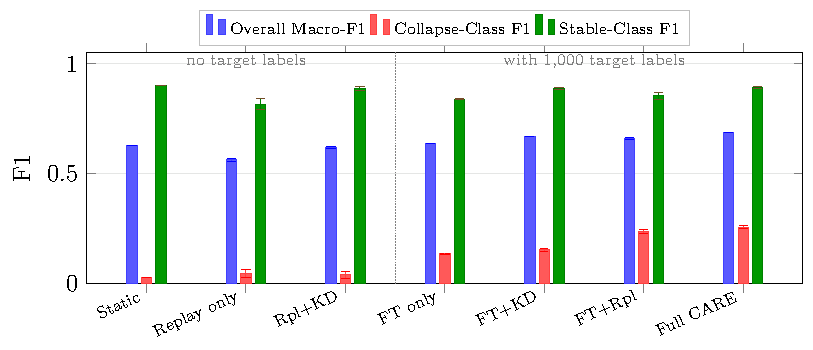
\includegraphics[width=\textwidth]{fig_ablation_bar.pdf}
\fi
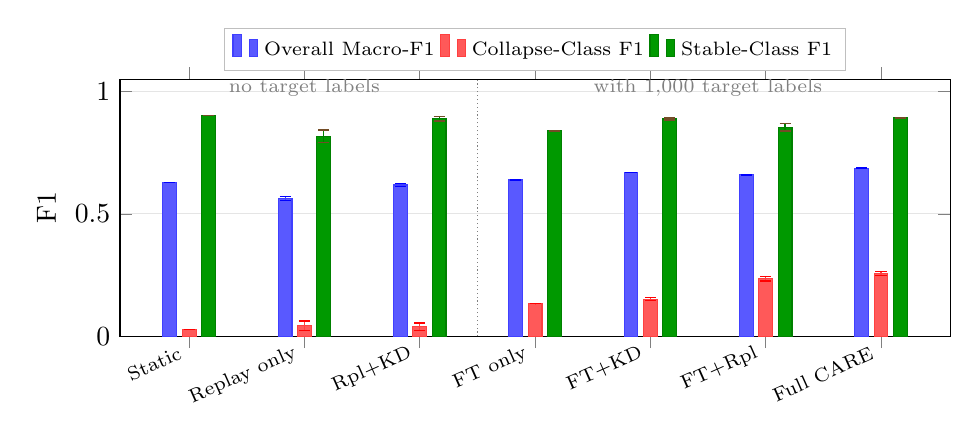
\begin{tikzpicture}
\begin{axis}[
  ybar,
  width=\textwidth,
  height=0.40\textwidth,
  ymin=0,
  ymax=1.05,
  ylabel={F1},
  xtick={0,1,2,3,4,5,6},
  xticklabels={Static,Replay only,Rpl+KD,FT only,FT+KD,FT+Rpl,Full CARE},
  x tick label style={rotate=24,anchor=east,font=\scriptsize},
  ymajorgrids,
  grid style={gray!20},
  legend style={at={(0.5,1.03)},anchor=south,legend columns=3,font=\scriptsize,draw=gray!50,fill=white},
  bar width=5pt,
  enlarge x limits=0.10,
]
\addplot+[fill=blue!65,draw=blue!75,/pgfplots/error bars/y dir=both,/pgfplots/error bars/y explicit] coordinates {
  (0,0.629) +- (0,0.000) (1,0.563) +- (0,0.007) (2,0.618) +- (0,0.005)
  (3,0.638) +- (0,0.000) (4,0.670) +- (0,0.000) (5,0.659) +- (0,0.003)
  (6,0.686) +- (0,0.001)};
\addplot+[fill=red!65,draw=red!75,/pgfplots/error bars/y dir=both,/pgfplots/error bars/y explicit] coordinates {
  (0,0.028) +- (0,0.000) (1,0.044) +- (0,0.019) (2,0.039) +- (0,0.016)
  (3,0.134) +- (0,0.001) (4,0.152) +- (0,0.007) (5,0.236) +- (0,0.010)
  (6,0.256) +- (0,0.009)};
\addplot+[fill=green!60!black,draw=green!50!black,/pgfplots/error bars/y dir=both,/pgfplots/error bars/y explicit] coordinates {
  (0,0.903) +- (0,0.000) (1,0.816) +- (0,0.026) (2,0.888) +- (0,0.009)
  (3,0.839) +- (0,0.001) (4,0.887) +- (0,0.004) (5,0.854) +- (0,0.016)
  (6,0.892) +- (0,0.003)};
\legend{Overall Macro-F1,Collapse-Class F1,Stable-Class F1}
\draw[densely dotted,gray] (axis cs:2.5,0) -- (axis cs:2.5,1.05);
\node[gray,font=\scriptsize] at (axis cs:1,1.015) {no target labels};
\node[gray,font=\scriptsize] at (axis cs:4.5,1.015) {with 1,000 target labels};
\end{axis}
\end{tikzpicture}
\caption{Original component bundles in Table~\ref{tab:ablation}. Full \ours{} has the highest macro-F1 and collapse F1 within this study. Typeset from the archived values with Codex-assisted LaTeX layout adjustments.}
\label{fig:ablation_bar}
\end{figure}
\FloatBarrier

Without target labels, replay-only rows leave collapse F1 below 0.05; adding distillation improves stable F1 from 0.816 to 0.888 but does not repair collapse. With target labels:
\begin{itemize}
  \item \textbf{FT only} raises collapse F1 from 0.028 to 0.134 but lowers stable F1 from 0.903 to 0.839.
  \item \textbf{FT+KD} restores stable F1 to 0.887, with collapse F1 of 0.152.
  \item \textbf{FT+Rpl} reaches 0.236 collapse F1 and 0.659 macro-F1, with stable F1 of 0.854.
  \item \textbf{Full \ours{}} reaches 0.686 macro-F1, 0.256 collapse F1, and 0.892 stable F1.
\end{itemize}
The evaluated bundles associate target supervision with collapse recovery and reference-based regularization with stable-class preservation. Because replay coverage and target repetition also vary, Table~\ref{tab:ablation} does not isolate each loss term. Supplementary Material S2 reports additional fixed-budget, matched-update controls on independently reconstructed public rows. Reference distillation without reference cross-entropy gives higher mean F1 and lower negative-flip rates than full CARE in those controls; full CARE avoids additional threshold-defined collapses in two BADGE seeds. These results qualify the incremental value of reference supervision, without replacing the original S-split results.

Fine-tuning depth.
We compare head-only repair (default) with full-model fine-tuning (encoder + head, learning rate scaled by $0.1{\times}$) under the same 1{,}000-label budget (Margin, all-class replay $k{=}5$, 5 seeds).
Full fine-tuning achieves macro-F1 of $0.678{\pm}0.001$ and collapse F1 of $0.256{\pm}0.005$, while head-only repair reaches $0.686{\pm}0.001$ and $0.256{\pm}0.009$, respectively.
Collapse recovery is comparable, but full fine-tuning slightly reduces overall and stable-class performance under the same label budget; this may reflect limited supervision for updating the encoder's ${\sim}$200K parameters.
The result supports freezing the encoder when the operational objective is a bounded repair under a small label budget.

\subsubsection{Selection Strategy Comparison}
\label{sec:al_baselines}

\begin{figure}[!htbp]
\centering
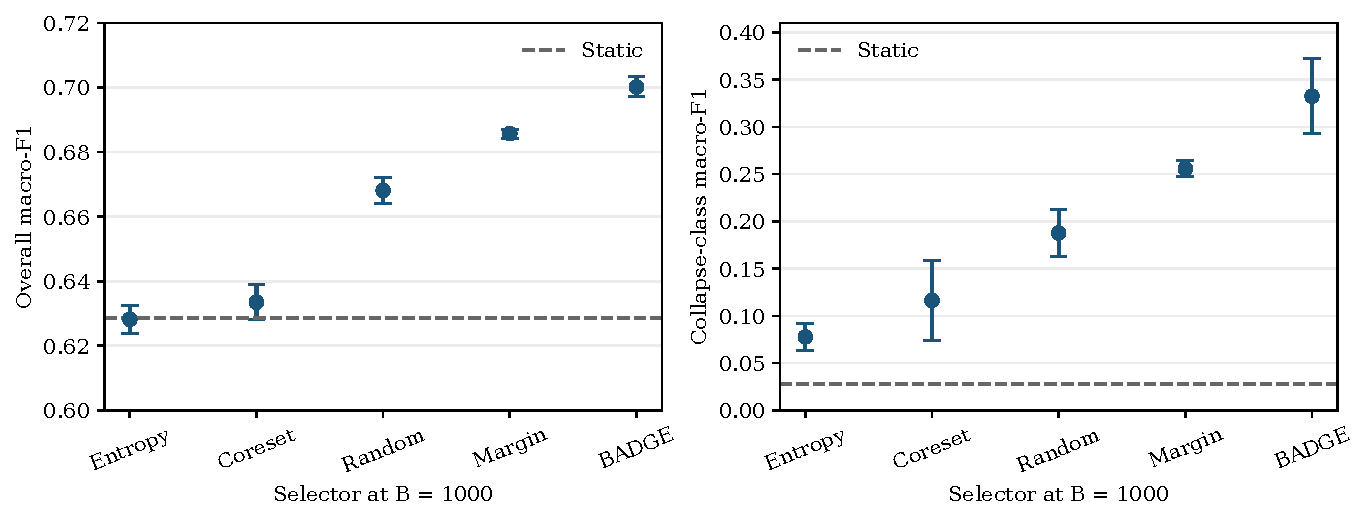
\includegraphics[width=\textwidth]{fig_strategy_comparison.pdf}
\caption{Selector comparison at $B{=}1{,}000$ with the same all-class replay and distillation pipeline (strict query exclusion; mean $\pm$ sample standard deviation over five repair seeds). Dashed lines show the static model. The plotted values correspond to Table~\ref{tab:main_results}; mean differences do not establish a definitive selector ranking. Replotted from archived numeric records using a Codex-assisted Matplotlib script.}
\label{fig:strategy_comparison}
\end{figure}
\FloatBarrier

The selector comparison is shown in Figure~\ref{fig:strategy_comparison}. Margin sampling selects globally low-margin samples, which may include absorber--victim boundaries.
BADGE~\cite{ash2020badge} achieves the highest collapse F1 ($0.332{\pm}0.040$), 30\% above Margin ($0.256{\pm}0.009$), and macro-F1 ($0.700{\pm}0.003$ vs.\ $0.686{\pm}0.001$).
BADGE has the higher mean performance when its selector complexity is acceptable, but the protocol-matched benchmark makes the trade-off explicit: \ours{}-BADGE is the slowest timed configuration at $166.6{\pm}8.2$\,s, about $3.4{\times}$ the $48.5{\pm}0.8$\,s required by \ours{}-Margin.

With a fixed selector (Table~\ref{tab:per_class_recovery}), Margin yields 4 recovered, 3 partial, and 5 failed classes, whereas BADGE yields 5 recovered, 5 partial, and 2 failed classes, using seed-mean recall under the strict protocol.
Both selectors allocate very few labels to collapse classes (0--13.6 per class on average out of 1{,}000). These cases indicate that recovery can arise from global boundary updates driven by target labels outside the affected class together with all-class replay, rather than direct labels for every collapsed class.

\begin{table}[!htbp]
\centering
\caption{Per-class recovery at M-2022-12 ($B{=}1{,}000$, all-class replay $k{=}5$, strict eval, 5 seeds; mean $\pm$ sample standard deviation). Selected = mean target labels allocated to that class.}
\label{tab:per_class_recovery}
\scriptsize
\setlength{\tabcolsep}{2pt}
\resizebox{\textwidth}{!}{%
\begin{tabular}{@{}r r r cc cc cc rr@{}}
\toprule
& & & \multicolumn{2}{c}{Static} & \multicolumn{2}{c}{\ours{}-Margin} & \multicolumn{2}{c}{\ours{}-BADGE} & \multicolumn{2}{c}{Selected} \\
\cmidrule(lr){4-5} \cmidrule(lr){6-7} \cmidrule(lr){8-9} \cmidrule(lr){10-11}
Class & Abs. & $n$ & Recall & F1 & Recall & F1 & Recall & F1 & Marg & BADGE \\
\midrule
56  & 96  & 12137 & 0.000 & 0.001 & 0.722$\pm$0.033 & 0.784$\pm$0.008 & \textbf{0.793$\pm$0.017} & \textbf{0.829$\pm$0.021} & 12.0 & 13.6 \\
163 & 46  &  1741 & 0.016 & 0.026 & 0.143$\pm$0.031 & 0.168$\pm$0.024 & \textbf{0.226$\pm$0.140} & \textbf{0.235$\pm$0.123} &  3.0 &  4.8 \\
174 &  2  &  1507 & 0.000 & 0.000 & \textbf{0.195$\pm$0.005} & \textbf{0.262$\pm$0.012} & 0.029$\pm$0.040 & 0.044$\pm$0.060 &  4.0 &  1.6 \\
48  & 14  &  3361 & 0.001 & 0.002 & 0.437$\pm$0.009 & 0.568$\pm$0.007 & \textbf{0.722$\pm$0.234} & \textbf{0.767$\pm$0.146} &  4.0 &  4.8 \\
38  & 45  &   193 & 0.052 & 0.090 & \textbf{0.656$\pm$0.095} & \textbf{0.410$\pm$0.057} & 0.242$\pm$0.277 & 0.210$\pm$0.210 &  3.0 &  1.2 \\
69  & 105 &  1866 & 0.005 & 0.008 & 0.031$\pm$0.017 & 0.042$\pm$0.021 & \textbf{0.157$\pm$0.203} & \textbf{0.177$\pm$0.219} &  3.0 &  2.4 \\
104 &  2  &  1744 & 0.010 & 0.016 & \textbf{0.703$\pm$0.044} & \textbf{0.664$\pm$0.031} & 0.604$\pm$0.154 & 0.594$\pm$0.073 &  8.0 &  3.6 \\
47  &  5  &   618 & 0.000 & 0.000 & 0.002$\pm$0.002 & 0.004$\pm$0.003 & \textbf{0.404$\pm$0.201} & \textbf{0.462$\pm$0.168} &  0.0 &  2.2 \\
66  & 71  &  1955 & 0.001 & 0.002 & 0.001$\pm$0.000 & 0.002$\pm$0.001 & \textbf{0.133$\pm$0.118} & \textbf{0.144$\pm$0.121} &  1.0 &  4.2 \\
10  & 156 &  1004 & 0.098 & 0.162 & 0.074$\pm$0.030 & 0.121$\pm$0.044 & \textbf{0.389$\pm$0.215} & \textbf{0.441$\pm$0.193} &  0.0 &  1.8 \\
109 & 71  &   393 & 0.000 & 0.000 & 0.000$\pm$0.000 & 0.000$\pm$0.000 & 0.000$\pm$0.000 & 0.000$\pm$0.000 &  0.0 &  1.6 \\
26  & 13  &   807 & 0.022 & 0.025 & 0.035$\pm$0.012 & 0.046$\pm$0.011 & \textbf{0.125$\pm$0.140} & \textbf{0.087$\pm$0.069} &  1.0 &  2.6 \\
\midrule
\multicolumn{3}{@{}l}{Macro (12 classes)} & 0.017 & 0.028 & 0.250 & 0.256 & \textbf{0.319} & \textbf{0.332} & & \\
\bottomrule
\end{tabular}%
}
\end{table}

\begin{figure}[!htbp]
\centering
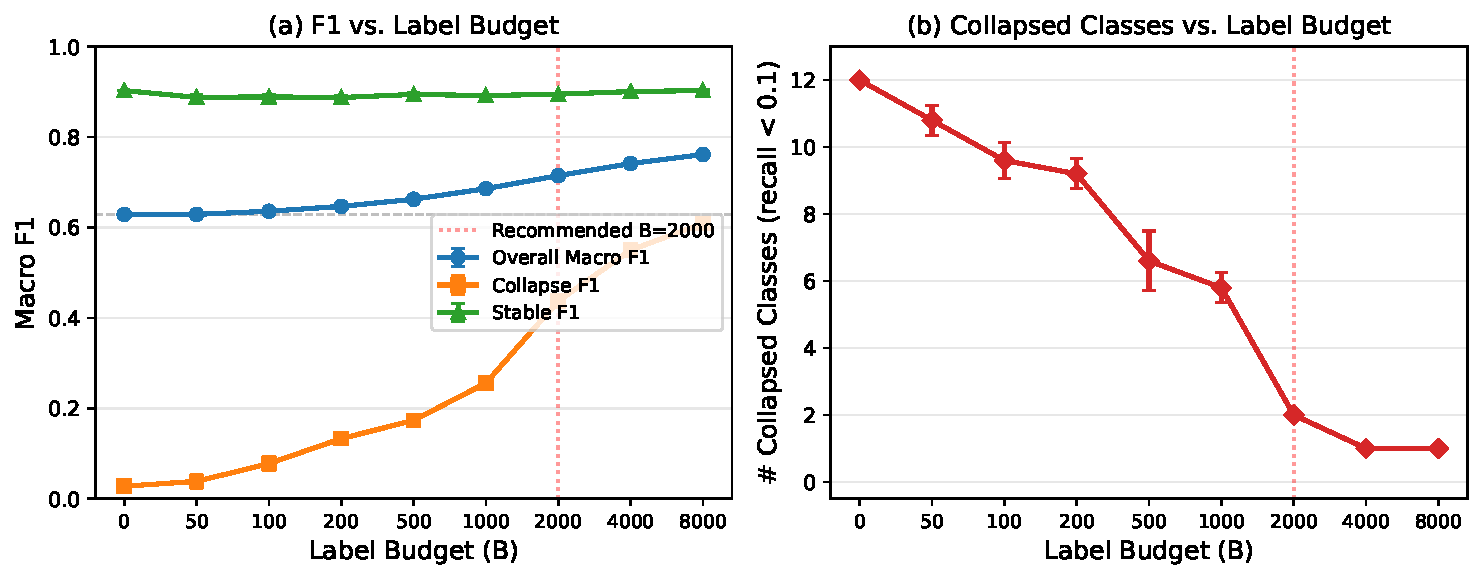
\includegraphics[width=\textwidth]{budget_curve.pdf}
\caption{Label budget vs.\ performance (margin, 5 seeds, error bars). Left: Overall, collapse, and stable macro F1. Right: number of collapsed classes (recall $< 0.1$). The knee at $B{=}2{,}000$ reduces collapsed classes from 12 to 2; beyond $B{=}4{,}000$ gains are marginal.}
\label{fig:budget_sweep}
\end{figure}
\FloatBarrier

Figure~\ref{fig:budget_sweep} shows performance across label budgets from $B{=}0$ to $B{=}8{,}000$.
Collapse F1 improves steadily from 0.028 (static) to $0.609{\pm}0.007$ at $B{=}8{,}000$, while stable-class F1 remains at least 0.887; this limits, but does not eliminate, degradation relative to the 0.903 static stable-class F1.
$B{=}2{,}000$ is an empirical knee: it raises collapse F1 to $0.437{\pm}0.004$ (a $16{\times}$ improvement over static) and reduces collapsed classes from 12 to 2, although the preferred operating point depends on local annotation cost.
Beyond $B{=}4{,}000$ ($0.550{\pm}0.007$), gains are marginal ($+0.015$ per additional 1{,}000 labels vs.\ $+0.181$ in the 1{,}000$\to$2{,}000 range).
All labeled CARE, active-learning, and continual-learning comparisons use $B{=}1{,}000$. Chen-style rows use no human labels and a separate pseudo-label regime; the budget curve shows how larger human-label budgets affect CARE.

\subsubsection{Replay Strategy Comparison}
\label{sec:replay_ablation}

A key design choice is whether to replay all classes or only detected/targeted classes.
Table~\ref{tab:replay_ablation} compares replay strategies under matched conditions (margin, $B{=}1{,}000$, 5 seeds).

\begin{table}[!htbp]
\centering
\caption{Replay strategy comparison (Margin, $B$=1000, 5 seeds). ``Targeted'' uses an oracle stable+absorber list; results support class-coverage breadth rather than replay volume as the explanation in this comparison.}
\label{tab:replay_ablation}
\scriptsize
\setlength{\tabcolsep}{3pt}
\begin{tabular}{@{}l cc c@{}}
\toprule
Replay Config. & Macro & Col.\ F1 & $n_{\text{rpl}}$ \\
\midrule
All-class $k{=}5$ (890) & \textbf{0.686$\pm$0.001} & \textbf{0.256$\pm$0.009} & 890 \\
Targeted $k{=}30$ (${\sim}$900) & 0.678$\pm$0.001 & 0.243$\pm$0.003 & $\sim$900 \\
All-class $k{=}1$ (178) & 0.680$\pm$0.003 & 0.231$\pm$0.015 & 178 \\
\bottomrule
\end{tabular}
\end{table}

All-class replay with $k{=}5$ yields the best results (0.686 macro-F1).
To assess whether all-class replay benefits only from using more features, we match the total replay budget: targeted replay with $k{=}30$ (${\approx}$900 features, matched budget) achieves 0.678, while all-class $k{=}1$ (178 features) achieves 0.680.
This comparison supports class-coverage breadth rather than replay volume as an explanation: anchoring all 178 class boundaries performs better than concentrating replay on a subset.

This finding also clarifies the role of the detection module.
Its intended value in the proposed deployment workflow is \textit{not} to guide replay class selection---all-class replay performs better in the tested ablation---but to (1)~flag classes at risk of degradation for operator investigation and (2)~indicate \textit{when} repair should be considered by the operator.

Prototype replay.
\label{sec:proto_replay}
In the tested targeted-replay variant, prototype replay retains 98.7\% of individual-exemplar macro-F1 ($0.664{\pm}0.002$ versus $0.673{\pm}0.001$) while reducing stored features from about 150~KiB to 60~KiB. This result shows that storage-efficient replay is feasible in the tested setting; formal privacy guarantees and validation in the default all-class configuration remain future work.

\subsection{Generalization and Robustness}
\label{sec:generalization_robustness}

This subsection examines whether the observed repair behavior persists across model architectures, transport protocols, and source-training and checkpoint variation.

\subsubsection{Architecture Robustness}
\label{sec:robustness}

\label{sec:bn_verify}
\label{sec:transformer}
To test whether normalization choice alone explains the TTA result, we train an otherwise identical CNN with Batch Normalization (BN): BN-Adapt~\cite{schneider2020bn} raises macro-F1 by only 0.009 while collapse F1 stays at 0.032, and NOTE degrades substantially (macro-F1: 0.042). A targeted-replay \ours{}-Margin variant improves the BN model (0.613$\to$0.665 macro, 0.030$\to$0.314 collapse).
We also train a Transformer backbone~\cite{vaswani2017attention} (4-layer, 4-head, 256-dim). Under the tested targeted-replay \ours{}-Margin protocol, it reaches $0.767{\pm}0.001$ macro-F1 and $0.401{\pm}0.003$ collapse F1. Because this replay protocol differs from the default all-class CNN experiment, we do not treat the gain magnitudes as a protocol-matched backbone comparison.

\subsubsection{Cross-Protocol Generalization}
\label{sec:cross_protocol}

QUICEXT-25 stress test.
\label{sec:quicext25}
To test whether the repair protocol transfers beyond TLS traffic, we evaluate \ours{} on the CESNET-QUICEXT-25 XS split~\cite{cesnetquicext25,mucke2025waiting}, a 44-class QUIC dataset with monthly partitions.
We train on M-2024-6 and evaluate on M-2025-5, where three drift-induced classes (17, 23, and 25) fall below 0.1 recall.
Class 21 also has near-zero target recall but is excluded because the model already fails to learn it in the reference period; it is not a drift-induced collapse case.

Table~\ref{tab:quicext25} reports a label-budget sweep.
Static macro-F1 is 0.502 and collapse-class F1 is 0.049.
With 1{,}000 queried target labels, \ours{}-Margin raises macro-F1 to $0.564{\pm}0.003$ and collapse F1 to $0.114{\pm}0.002$, reducing collapsed classes from 3.0 to 2.0.
Larger budgets are more effective on QUICEXT-25: \ours{}-BADGE at $B{=}4{,}000$ reaches $0.586{\pm}0.007$ macro-F1 and $0.191{\pm}0.030$ collapse F1, with collapsed classes reduced to $1.2{\pm}0.45$.
Here $B$ denotes the number of queried target labels, not the number of feature vectors used for head training.
With target repeat factor 2 and 220 all-class replay features, the $B{=}4{,}000$ setting uses 8{,}220 head-training feature vectors but only 4{,}000 newly labeled target samples.

\begin{table}[!htbp]
\centering
\caption{Cross-protocol generalization on CESNET-QUICEXT-25 XS (M-2024-6 $\to$ M-2025-5, 44 classes, 5 seeds). $B$ is the number of queried target labels; strict evaluation excludes them.}
\label{tab:quicext25}
\scriptsize
\setlength{\tabcolsep}{3pt}
\begin{tabular}{@{}l c c c c@{}}
\toprule
Method & $B$ & Macro-F1 & Collapse F1 & \#Col. \\
\midrule
Static & 0 & 0.502 & 0.049 & 3.0 \\
\ours{}-Margin & 1000 & $0.564{\pm}0.003$ & $0.114{\pm}0.002$ & $2.0{\pm}0.0$ \\
\ours{}-BADGE & 1000 & $0.563{\pm}0.006$ & $0.091{\pm}0.017$ & $2.8{\pm}0.45$ \\
\ours{}-Margin & 2000 & $0.577{\pm}0.003$ & $0.126{\pm}0.014$ & $2.0{\pm}0.0$ \\
\ours{}-BADGE & 2000 & $0.578{\pm}0.006$ & $0.144{\pm}0.031$ & $2.2{\pm}0.84$ \\
\ours{}-Margin & 4000 & $0.578{\pm}0.002$ & $0.132{\pm}0.021$ & $1.8{\pm}0.45$ \\
\ours{}-BADGE & 4000 & $\mathbf{0.586{\pm}0.007}$ & $\mathbf{0.191{\pm}0.030}$ & $\mathbf{1.2{\pm}0.45}$ \\
\bottomrule
\end{tabular}
\end{table}

The QUICEXT-25 stress test demonstrates positive cross-protocol transfer: \ours{} improves both macro-F1 and collapse F1 while reducing the number of collapsed classes. The strongest tested setting, \ours{}-BADGE with $B{=}4{,}000$, reaches macro-F1 of $0.586{\pm}0.007$ and collapse F1 of $0.191{\pm}0.030$, with collapsed classes reduced to $1.2{\pm}0.45$. The larger label requirement defines a different QUIC operating point rather than a failure of transfer and motivates protocol-aware maintenance budgets.

\subsubsection{Training-Seed and Checkpoint Robustness}
\label{sec:checkpoint_robustness}

A targeted-replay retraining audit ($3{\times}3{=}9$ runs) yields static macro-F1 of $0.620{\pm}0.001$ and CARE macro-F1 of $0.667{\pm}0.007$ across training seeds.
Our primary checkpoint (static $0.629$, best epoch 27/30, validation F1 $0.892$) is about 0.009 above the audit mean, larger than the audit standard deviation and therefore evidence of checkpoint/run sensitivity. The targeted-replay CARE variant improves over its corresponding static model in all audited training seeds, although the gain magnitude varies.

\subsection{Diagnostic Detector Evaluation}
\label{sec:detection_eval}

Signal ablation.
Table~\ref{tab:detect_signals} shows how each signal contributes to detection performance at M12.
The detection ground truth uses the same collapse definition as repair evaluation: recall~${<}\,0.1$ with support~${\geq}\,50$, yielding 12 ground-truth collapsed classes.
The detector selects the 20 highest-risk classes ($k{=}20$).

\begin{table}[!htbp]
\centering
\caption{Detection signal ablation on M4$\to$M12 (12 ground-truth classes, no target labels used by the detector, $k{=}20$). Count denotes prediction-count drop; FD denotes Fr\'{e}chet distance.}
\label{tab:detect_signals}
\small
\begin{tabular}{@{}l ccc@{}}
\toprule
Signal Combination & Precision & Recall & F1 \\
\midrule
FD only & 0.350 & 0.583 & 0.438 \\
Count + FD & 0.450 & 0.750 & 0.563 \\
Count + FD + margin + confidence & 0.400 & 0.667 & 0.500 \\
All 5 signals & \textbf{0.500} & \textbf{0.833} & \textbf{0.625} \\
\bottomrule
\end{tabular}
\end{table}

Count drop and FD provide a strong two-signal baseline (F1 = 0.563). Relative to the four-signal row, adding entropy rise lifts recall from 0.667 to 0.833 and F1 from 0.500 to 0.625.

Detection across drift levels.
Table~\ref{tab:trigger} evaluates detection consistency as a diagnostic monitor across four time points.

\begin{table}[!htbp]
\centering
\caption{Detection across drift levels ($k{=}20$, recall${<}0.1$, support${\geq}50$). GT denotes ground truth; recall is $\geq$0.80 throughout.}
\label{tab:trigger}
\small
\begin{tabular}{@{}l cccc@{}}
\toprule
Period & GT & Precision & Recall & F1 \\
\midrule
M7 (light)   & 5  & 0.200 & 0.800 & 0.320 \\
M9 (medium)  & 8  & 0.350 & 0.875 & 0.500 \\
M11 (heavy)  & 10 & 0.450 & 0.900 & 0.600 \\
M12 (severe) & 12 & 0.500 & 0.833 & 0.625 \\
\bottomrule
\end{tabular}
\end{table}

Recall is $\geq$0.80 at all periods; precision rises from 0.20 at M7 to 0.50 at M12, coinciding with an increase in ground-truth collapsed classes.
At M12, the two missed classes are 38 (small support) and 163 (gradual drift).

Detection weight sensitivity.
The manual weights achieve the best observed detection F1 of 0.625 without labeled calibration and match the calibrated weights on M12 (precision 0.50, recall 0.83). Equal weights remain competitive at F1 0.563. The close results across manual, equal, and calibrated settings show that the detector is not highly sensitive to exact weighting over the tested range.

% ============================================================
\section{Discussion}
\label{sec:discussion}

This section interprets the empirical findings, outlines their deployment implications, and delineates the study's limitations and directions for future work.

\subsection{Understanding the Efficacy of \ours{}}
\label{sec:discussion_efficacy}

Mechanism and stable-class preservation.
The original component bundles associate target labels with repair and reference-based regularization with stable-class preservation. Under the original protocol, CARE raises collapse-class F1 from 0.028 to 0.256 with Margin and 0.332 with BADGE, with stable-class F1 of 0.892 and 0.894 versus 0.903 for the static model. The component study and the separately reconstructed controls in S2 support assessment of the repair framework, but do not establish that reference cross-entropy is independently beneficial or necessary. The fine-tuning-depth comparison in Section~\ref{sec:ablation} further supports bounded head repair under the evaluated 1{,}000-label budget.

Why adjacent methods are insufficient.
The empirical gap is not simply a lack of generic adaptation. Entropy- and pseudo-label-based TTA receives little corrective signal when an absorber makes confident but wrong predictions, whereas continual-learning and drift-adaptation baselines primarily target new classes, forgetting, or global objectives. \ours{} instead couples a collapse-specific diagnostic with verified target labels and preservation constraints. The comparison is not cost- or supervision-matched in every case, but the consistently near-zero collapse F1 of tested label-free methods and the weaker recovery of generic active selectors support the evaluated use of verified labels and preservation-aware maintenance for class repair.

Generalization of the observed effect.
\ours{} improves macro-F1 at every evaluated TLS drift period and remains effective with CNN and Transformer backbones; the QUICEXT-25 stress test further shows that the repair principle transfers beyond TLS, although larger budgets are needed there. These results support robustness to the tested drift severity, architecture, and protocol changes, but they do not establish universal transfer across networks or organizations. The strongest claim supported by the evidence is therefore that collapse-aware, label-efficient repair is reusable across the evaluated settings, not that one fixed configuration is universally optimal.

Selector effectiveness and cost.
Finally, the choice of active selector determines how effectively the limited label budget is used. BADGE's higher mean performance than Margin is consistent with its selection of diverse, boundary-informative samples across multiple potential collapse regions. However, the BADGE configuration has about $3.4{\times}$ the program wall time ($166.6{\pm}8.2$\,s versus $48.5{\pm}0.8$\,s on one NVIDIA L20), and corrected significance tests do not establish a definitive ranking. Margin therefore remains attractive when latency and simplicity matter, whereas BADGE offers stronger mean recovery when the additional computation is acceptable.

\subsection{Practical Considerations for Deployment}
\label{sec:discussion_deployment}

Label acquisition and maintenance scope.
\ours{} requires 1{,}000 target labels per repair cycle (0.076\% of M12 and 0.094\% of the matched adaptation pool) plus 890 stored reference features. Depending on local policy, those labels could be obtained from DPI-assisted labeling on a monitored subnet, exposed SNI metadata, or manual verification using endpoint and domain records. A detector alert should initiate operator review rather than automatic retraining, so annotation is incurred only after a repair cycle is approved. This study did not measure human annotation time or monetary cost.

Operator-reviewed workflow.
An illustrative deployment could run \ours{} as a scheduled offline maintenance job beside the live classifier. The production model would continue serving predictions while the detector aggregates class-health statistics; an approved alert would authorize a limited label budget, after which a candidate classification head could be repaired on a separate machine, validated, versioned, and activated with rollback available. A monthly cycle matches the granularity evaluated here, but shorter monitoring windows, live acceptance gates, and integration with production traffic-analysis systems remain unvalidated.

Detection and operating trade-offs.
The detector maintains recall of at least 0.80 across evaluated periods, but M12 precision is 0.50, so screening favors sensitivity and imposes review cost through false alerts. This behavior is appropriate for a diagnostic monitor only if operators validate alerts before labeling and repair; otherwise, false positives could trigger unnecessary work. Once a cycle is approved, active selection and replay can address several collapse regions together, but recovery of every class is not guaranteed. The downstream value for traffic accounting, security triage, and capacity planning must therefore be established in a field study with application-specific error costs.

\subsection{Limitations and Future Work}
\label{sec:discussion_limitations}

Technical limitations.
Head-only repair cannot recover a class if its encoder representation has fully merged with an absorber; selective encoder adaptation or retraining may be required for such cases at higher cost. \ours{} repairs existing classes and does not address emerging classes, which require complementary class-incremental mechanisms~\cite{cai2024cpn}. S2 varies the reference month on one reconstructed December pool; sensitivity on the original S split and independent target periods remains untested. Prototype replay was evaluated only in a smaller targeted-replay variant; neither stored exemplars nor prototypes currently provide a formal privacy guarantee.

External validity and future work.
The primary evidence comes from university-network TLS traffic, while QUICEXT-25 is a cross-protocol stress test rather than a second full benchmark. Cross-site replication, longer operational studies, and direct measurement of annotation and review costs are needed before production claims can be made. Future work should calibrate detector thresholds against deployment-specific false-alert costs, study adaptive maintenance schedules, evaluate privacy-preserving replay, and invoke encoder adaptation only when bounded head repair fails. These studies would test this trade-off under heterogeneous traffic and policies.


% ============================================================
\section{Conclusion}
\label{sec:conclusion}

Reliable encrypted traffic classification requires tracking failures that aggregate metrics can conceal. We formalize absorber collapse, in which dominant classes absorb predictions from shifted victim classes. On CESNET-TLS-Year22, 12 of 178 classes collapse within nine months. \ours{} combines diagnostic monitoring with active target-label selection, all-class reference replay, knowledge distillation, and head-only repair to evaluate recovery alongside stable-class preservation.

Under strict query-excluded evaluation, \ours{}-BADGE raises macro-F1 from 0.629 to $0.700{\pm}0.003$ and collapse-class F1 from 0.028 to $0.332{\pm}0.040$ using 1{,}000 target labels and 890 replay features, while retaining stable-class F1 of 0.894. Tested TTA variants leave collapse F1 below 0.031. On seed-matched holdouts, our Chen-inspired self-evolving implementation leaves all 12 collapsed classes below the recall threshold. These comparisons support the value of verified target labels for this failure mode; they do not equate the methods' supervision or update budgets.

The component evidence supports evaluating target supervision with reference-based preservation, while the controls in S2 qualify the incremental value of reference cross-entropy. It does not establish that every loss term is necessary. Positive gains across the tested drift periods and backbones support reuse within these settings; the QUIC stress test exposes limits under a different protocol. CARE therefore offers an empirically supported maintenance framework for class-level prediction reliability. Fully merged representations, emerging classes, source-period sensitivity, cross-site validation, annotation cost, and privacy-preserving replay remain open issues.

\section*{CRediT Author Contribution Statement}
\textbf{Junwei Xiao}: Methodology; Software; Validation; Formal analysis; Writing -- original draft.
\textbf{Xiaobo Jin}: Supervision; Writing -- review and editing.
\textbf{Xiucheng Wu}: Validation; Writing -- review and editing.
\textbf{Dongjie Liu}: Supervision; Writing -- review and editing; Resources.

\section*{Funding}
This research did not receive any specific grant from funding agencies in the public, commercial, or not-for-profit sectors.

\section*{Data and Code Availability}
The experiments use the public CESNET-TLS-Year22 dataset~\cite{hynek2024cesnet}, available at \url{https://doi.org/10.5281/zenodo.10608607}, and CESNET-QUICEXT-25~\cite{cesnetquicext25,mucke2025waiting}, available at \url{https://doi.org/10.5281/zenodo.17249078}. Supplementary Material S1 is deposited in Figshare and is accessible for peer review via \url{https://figshare.com/s/bf40e243e93c5b2ac085}. S1 provides implementation files, configurations, archived experiment records, and available source checkpoints. Its result index maps manuscript tables and figures to the corresponding records and distinguishes strict query-excluded metrics from full-pool metrics. The original submission archive remains accessible via \url{https://figshare.com/s/7389bbfe6e00ae57d7ea}; it is a separate legacy archive. Both Figshare links provide private peer-review access rather than public DOIs.

Raw traffic datasets are distributed through the public repositories cited above and are not repackaged in S1. The original exact size-S row identities and full feature caches are unavailable. The archived materials support verification against the saved experiment records but do not provide a complete end-to-end reproduction of the original experiments. Supplementary Material S2 reports the separate reconstruction controls. Their frozen queries, selected training and reference features, fitted heads, per-class records, and provenance are included under \texttt{local\_controls/} in S1. These controls use independently reconstructed row identities and a reconstructed class mapping and are not substituted for the original size-S results.

\section*{Declaration of Generative AI and AI-Assisted Technologies in the Manuscript Preparation Process}
During preparation of this resubmission, OpenAI Codex assisted with language editing, organization of submission materials, and reproducible Matplotlib rendering from archived numeric records. It also assisted with implementing, executing, and verifying the separate reconstruction controls summarized in Supplementary Material S2. The original main-table results are retained and the additional controls are identified as a distinct protocol. The authors are responsible for reviewing the final text, code, and results and for the accuracy and integrity of the article.

\bibliographystyle{elsarticle-harv}
\bibliography{references}

\end{document}
